\documentclass{beamer}
\usetheme{Boadilla}
\setbeamertemplate{navigation symbols}{}
\setbeamercovered{invisible}
\useinnertheme{rounded}

%Palatino + AMS Euler
\usepackage[euler-digits,euler-hat-accent]{eulervm}
\usefonttheme{serif}
\usepackage{fontspec}
%\setmainfont{TeX Gyre Pagella}


\usepackage{tikz}
\usepackage{tikzscale}
\usetikzlibrary{shapes,arrows.meta}
\usetikzlibrary{positioning}
\usetikzlibrary{math}
\usetikzlibrary{external}
\tikzexternalize[optimize=false,prefix=tikz/]
\usepackage{amssymb}
\usepackage{nicefrac}
\usepackage{amsmath}
\usepackage{siunitx}
\usepackage{mathtools}
\usepackage{booktabs}
\usepackage{graphicx}
\sisetup{range-phrase=~...~}
\usepackage{pgfgantt}
\usepackage{soul}
\usepackage{pgfplots}
\pgfplotsset{compat=newest}
\usepgfplotslibrary{fillbetween}
\usepgfplotslibrary{groupplots}
\usepackage{listings}
\usepackage{tabularx}
\usepackage{subfig}

\definecolor{juasblue}{rgb}{0,0.5411,0.7647}
\definecolor{juasgrey}{rgb}{0.49,0.698,0.761}
\graphicspath{ {./img/}}

\title[Practical Days - RF]{CERN practical days - RF}
\subtitle{09:00} 
\author[Heine, Noll]{Ruben Heine \and Marvin Noll}
\date[\today]{14.03.2022}

\makeatletter
\colorlet{beamer@blendedblue}{juasblue}
\makeatother

\begin{document}
\begin{frame}[plain]
  \titlepage
\end{frame}

\begin{frame}{Outline}
    \tableofcontents
\end{frame}

\section{Forenoon Session}
\subsection{Band Pass Filter}
\begin{frame}[t,fragile]{Band Pass Filter (1) - Transmission $S_{12}$, $S_{21}$}
\begin{figure}
  \centering
  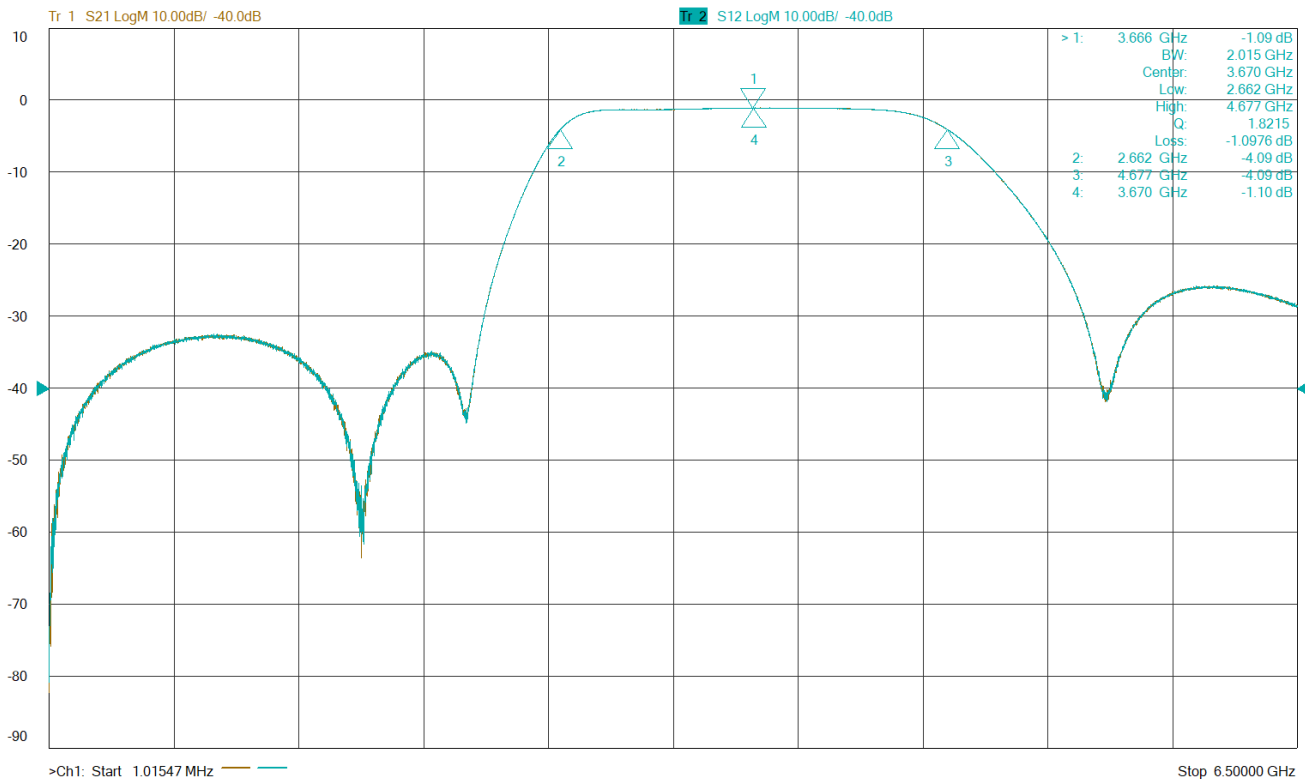
\includegraphics[width=0.9\textwidth]{img/bandpass_S12.png}
\end{figure}
\begin{equation*}
BW=\SI{2.015}{\GHz},\quad f=\SIrange{2.66}{4.67}{\GHz}
\end{equation*}
\begin{center}
$S_{21} \approx S_{12} \Rightarrow$ Reciprocal
\end{center}
\end{frame}

\begin{frame}[t,fragile]{Band Pass Filter (2) - Input/Output Reflection $S_{11}$, $S_{22}$}
\begin{figure}
  \centering
  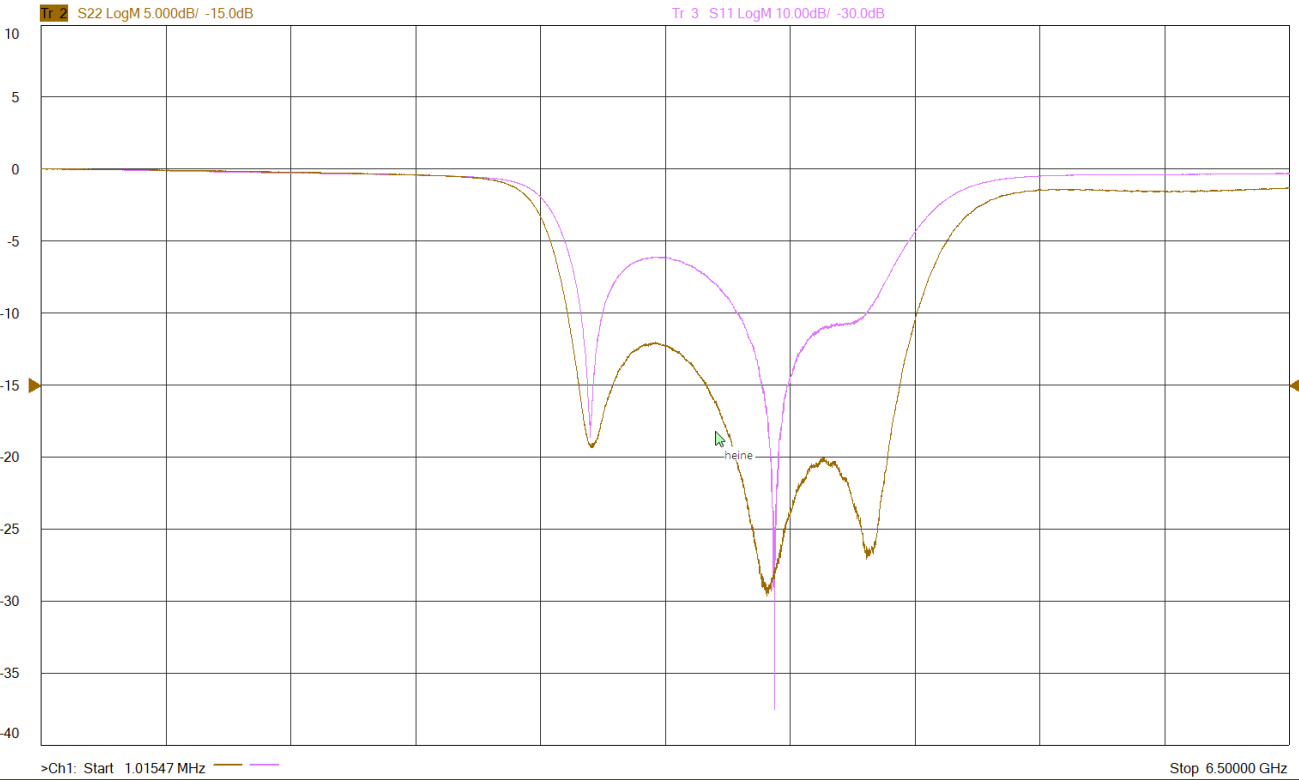
\includegraphics[width=0.9\textwidth]{img/bandpass_S11S22.png}
\end{figure}
\begin{center}
$S_{11} \neq S_{22} \Rightarrow$ Non symmetric
\end{center}
\end{frame}

\begin{frame}[t,fragile]{Band Pass Filter (3) - Phase $\angle S_{12}$}
\begin{figure}
  \centering
  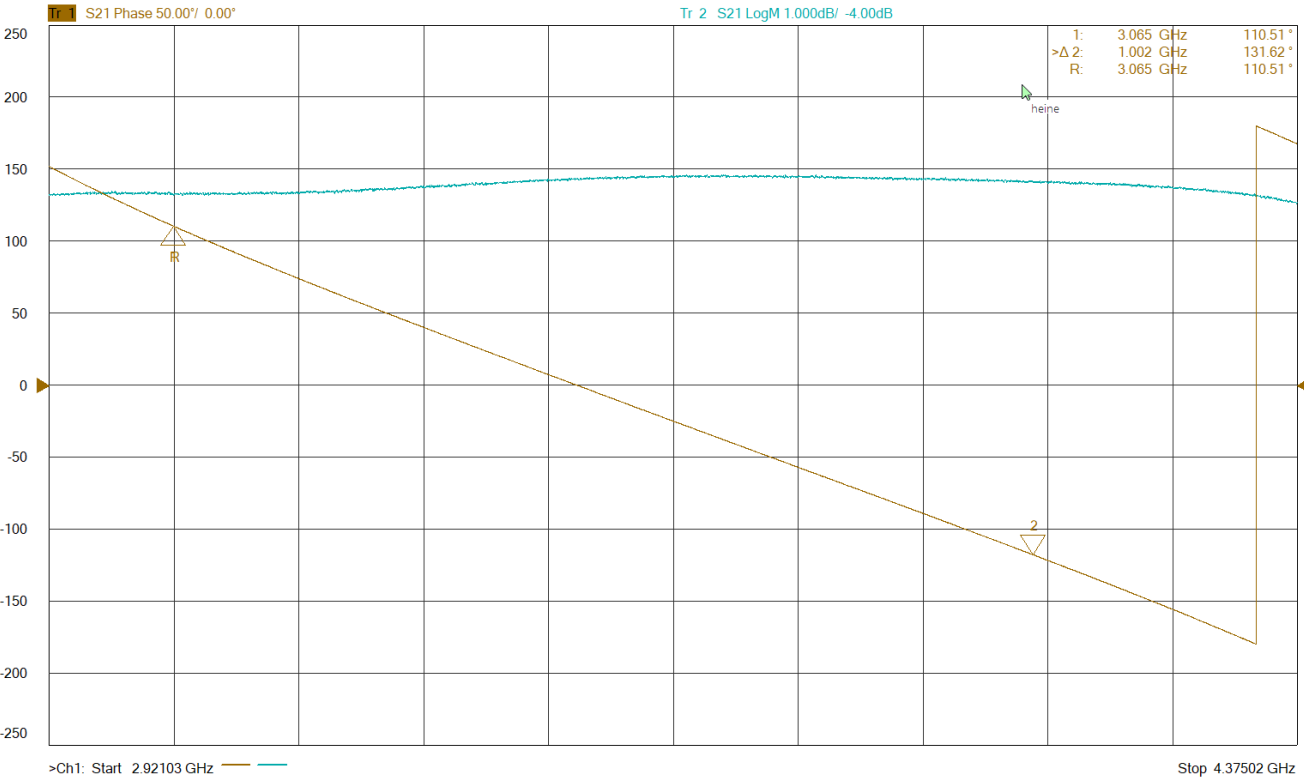
\includegraphics[width=0.9\textwidth]{img/bandpass_phase.png}
\end{figure}
\begin{equation*}
t_g = - \frac{\text{d}}{\text{d}\omega} \angle S_{12} \approx -\frac{\Delta \angle S_{12} \;[\si{\radian}]}{\Delta \omega} = \frac{(\SI{360}{\degree}-\SI{131.62}{\degree})\cdot \nicefrac{\pi}{180}}{2\pi\cdot\SI{1.002}{\GHz}} = \SI{633}{\pico\second}
\end{equation*}
\end{frame}

\begin{frame}[t,fragile]{Band Pass Filter (4) - Group Delay $t_g$}
\begin{figure}
  \centering
  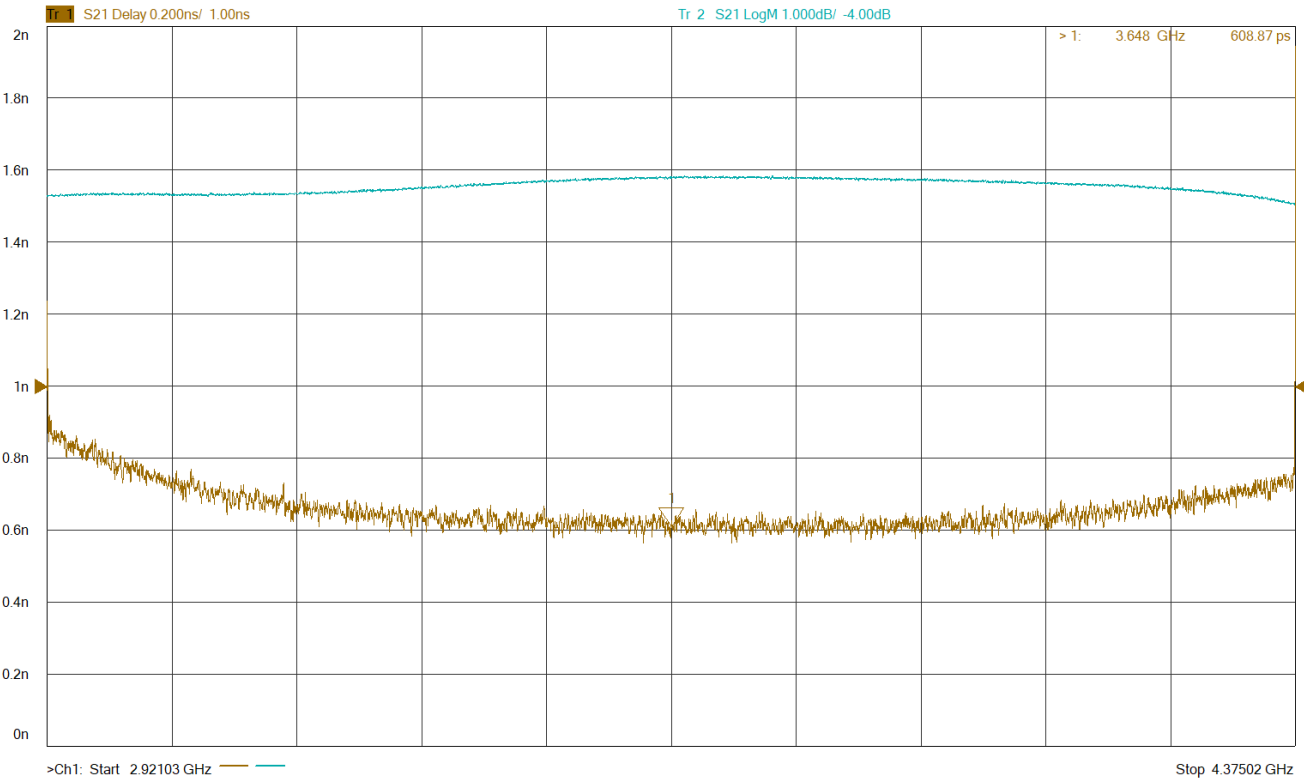
\includegraphics[width=0.9\textwidth]{img/bandpass_groupdelay.png}
\end{figure}
\begin{equation*}
\text{From group delay plot: }t_g = \SI{608.87}{\pico\second}
\end{equation*}
\end{frame}


\subsection{Strip-Line BPM}
\begin{frame}[t,fragile]{Strip-Line BPM (1) - Intro}

Reflectometry for \SI{500}{\MHz} and \SI{50}{\ohm}
\begin{itemize}
\item[a] Connector
\item[b] Strip line
\begin{itemize}
\item Four \SI{14}{\cm} strips
\item Short-circuit termination
\end{itemize}
\end{itemize}

\begin{figure}
  \centering
  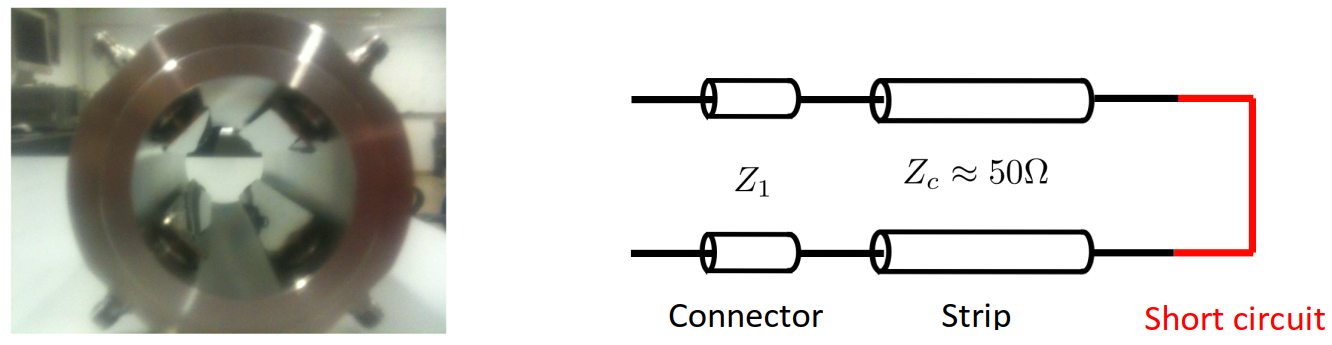
\includegraphics[width=0.9\textwidth]{2_1}
  \caption{Strip line: Photo and Circuit}
\end{figure}

\end{frame}

\begin{frame}[t,fragile]{Strip-Line BPM (2) - Time Domain Reflectometry}
\begin{itemize}
\item Measuring $S_{11}$ in time domain to check acceptance criteria
\begin{itemize}
\item[a] Connector: $+\SI{50}{mU}$ 
\item[b] Strip line: $\pm\SI{20}{mU}$
\end{itemize}
\item Strip line \textit{blue} in specs, \textit{gold} not in specs
\end{itemize}

\begin{figure}
  \centering\setcounter{subfigure}{0}
  \subfloat[TDR Aim]{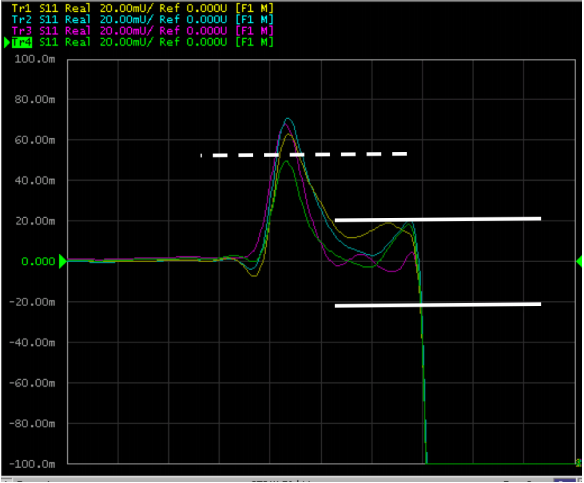
\includegraphics[width=0.4\textwidth]{2_2}}\quad
  \subfloat[TDR Reproduced]{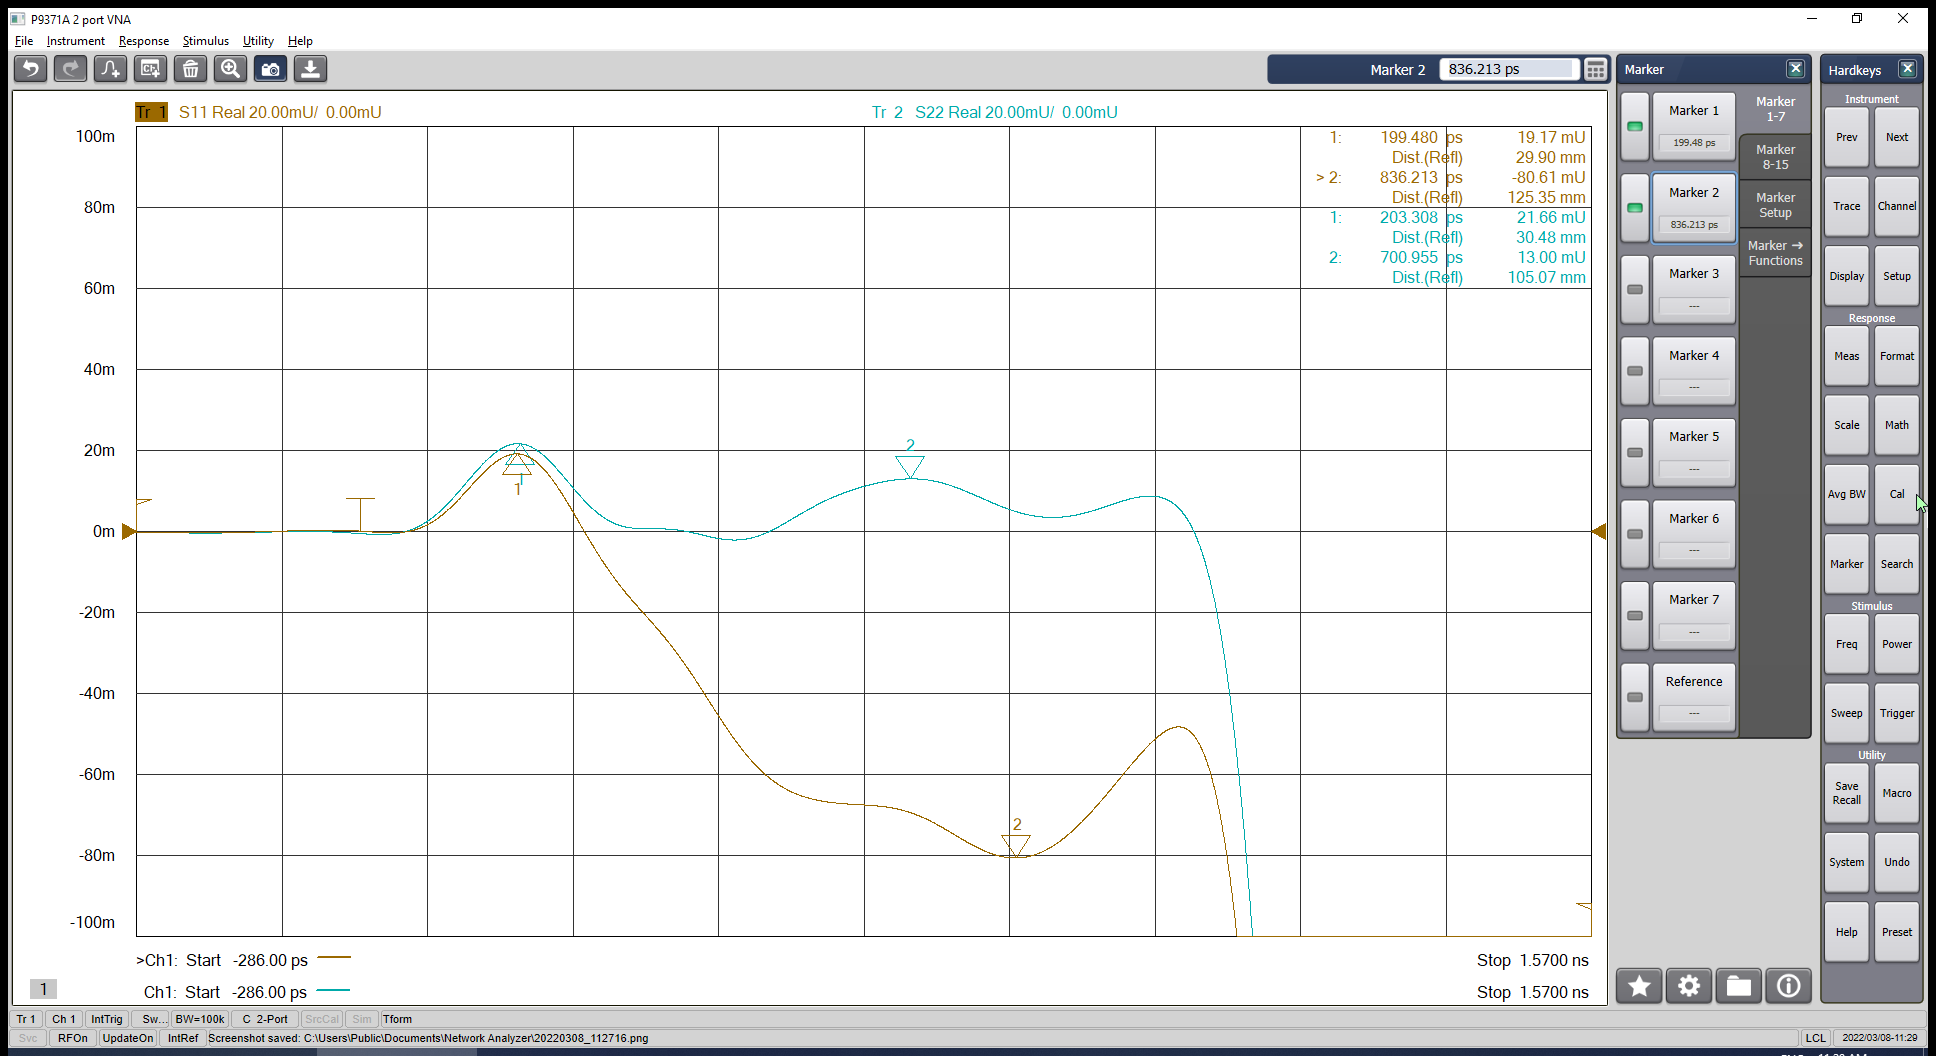
\includegraphics[width=0.55\textwidth]{2_S11_TD}}\\
\end{figure}

\end{frame}

\begin{frame}[t,fragile]{Strip-Line BPM (3) - Frequency Domain Characterization}
\begin{itemize}
\item Strip-line length from $S_{11}$
\begin{itemize}
\item from $S_{11}$: \SI{1.086}{\nano\second}, \SI{162.77}{\mm}
\item from phase: \SI{1.218}{\nano\second}, \SI{182.58}{\mm}
\item from group delay: \SI{1.32}{\nano\second}, \SI{197.87}{\mm}
\end{itemize}
\item Cross-talk from $S_{21}$
\begin{itemize}
\item Maximum transmission of \SI{-25.25}{\dB} at \SI{797.68}{\MHz}
\item Transmission of \SI{-53.06}{\dB} at operation frequency \SI{500}{\MHz}
\end{itemize}
\end{itemize}

\begin{figure}
  \centering\setcounter{subfigure}{0}
  \subfloat[Calculation from $S_{11}$]{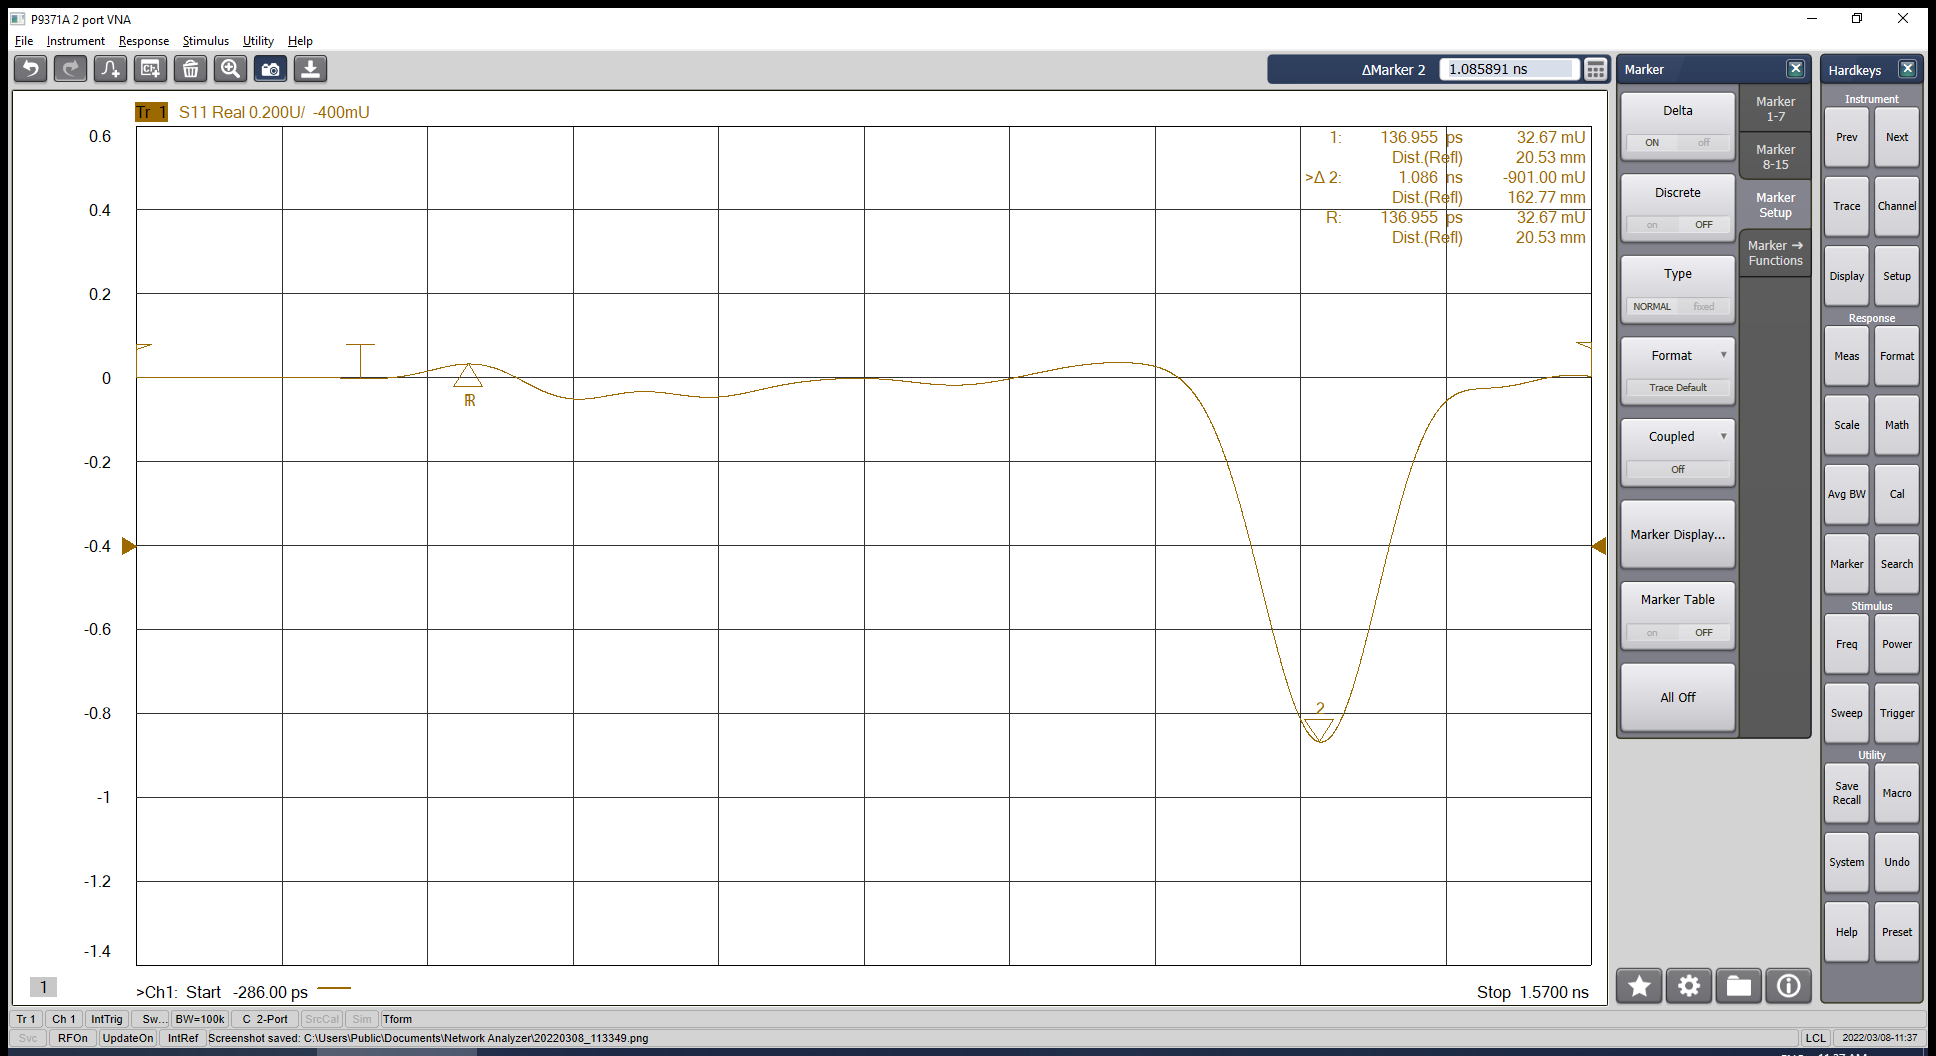
\includegraphics[width=0.48\textwidth]{2_length}}\quad
  \subfloat[Calculation from phase]{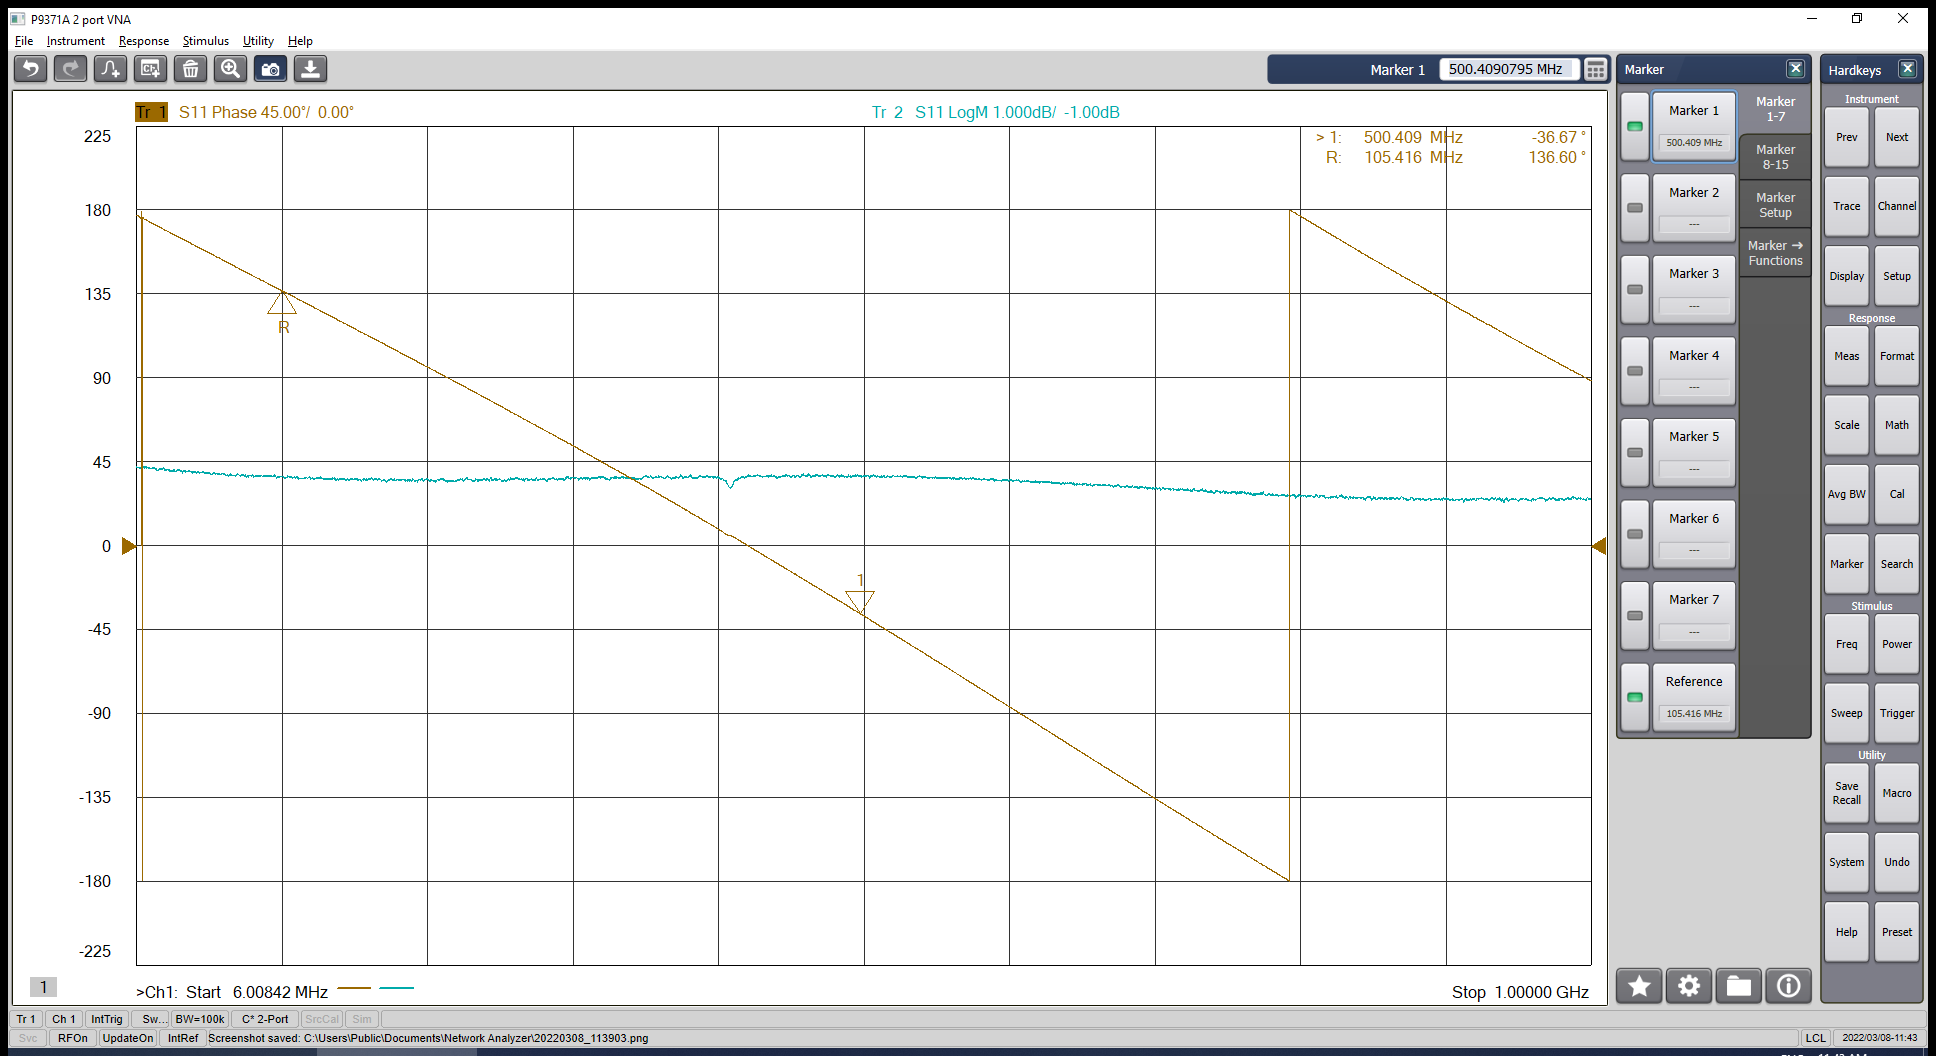
\includegraphics[width=0.48\textwidth]{2_phase}}\\
\end{figure}

\end{frame}

%\begin{frame}[t,fragile]{Strip-Line BPM (4) - Strip Line Length}
%\begin{itemize}
%\item Strip-line length from S11
%\begin{itemize}
%\item $1.086 ns$ translates to $162.77 mm$
%\end{itemize}
%\item Comparision with group delay: $1.218 ns$, $182.58 mm$
%\item Cross-talk from S21
%\begin{itemize}
%\item Maximum reflection of $ -25.25 dB$ at $797.68 MHz$ 
%\item Reflection of $ -53.06 dB$ at operation frequency $ 500.00 MHz$
%\end{itemize}
%\end{itemize}
%
%\begin{figure}
%  \centering
%  \subfloat[TDR Aim]{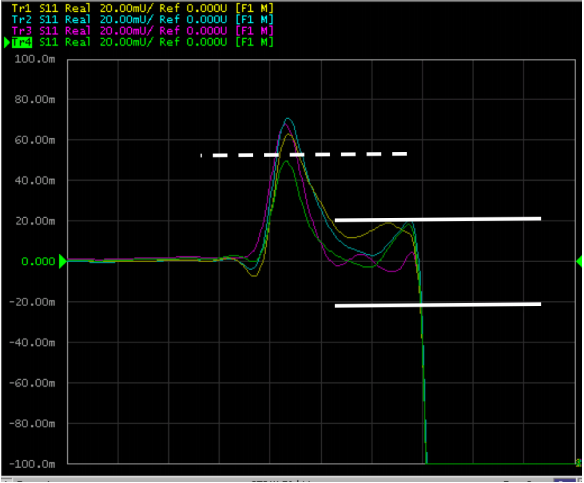
\includegraphics[width=0.4\textwidth]{2_2}}\quad
%  \subfloat[TDR Reproduced]{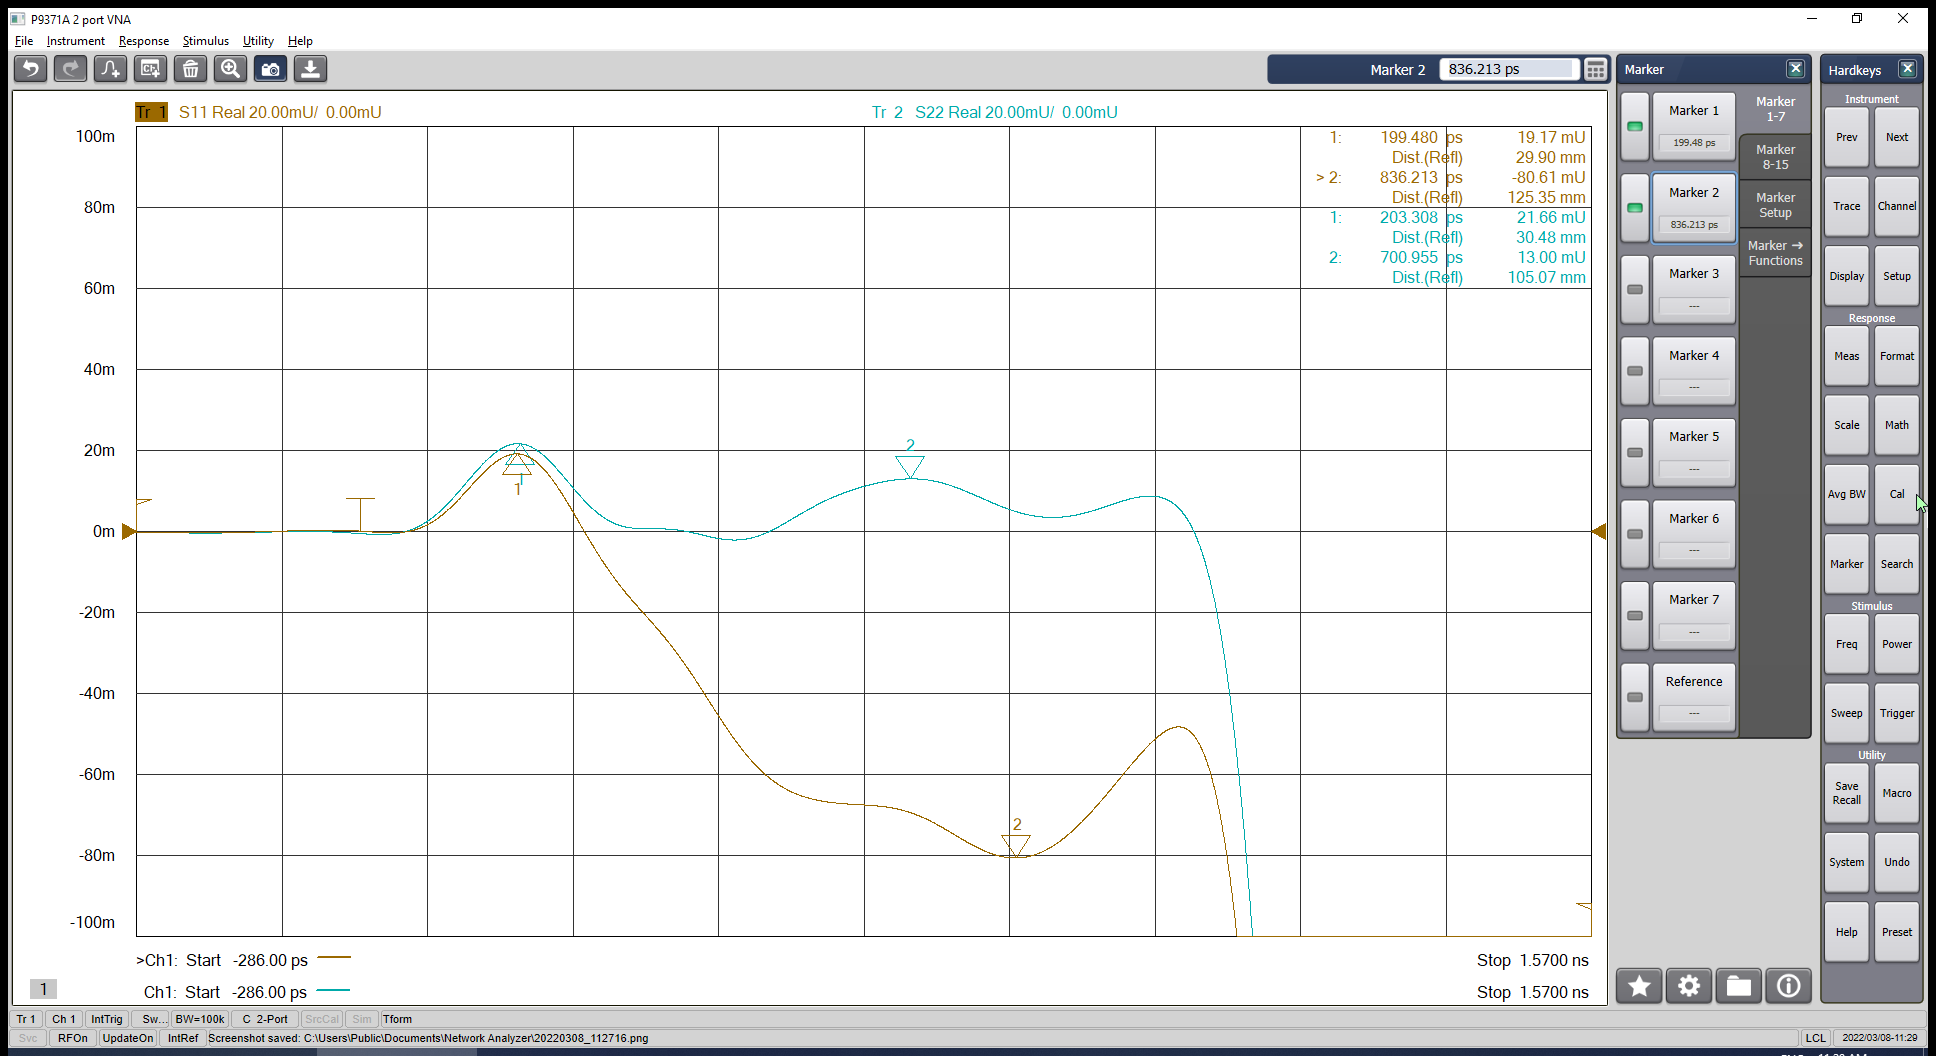
\includegraphics[width=0.55\textwidth]{2_S11_TD}}\\
%\end{figure}
%
%\end{frame}

\subsection{RF - Cavities}
\begin{frame}[t,fragile]{RF - Cavities (1) - Intro}
\begin{itemize}
\item Multi cell cavity in X-band
\item Operating mode at \SI{11.424}{\GHz}
\item Under coupled antenna
\end{itemize}

\begin{figure}
  \centering\setcounter{subfigure}{0}
  \subfloat[Multi cell cavity]{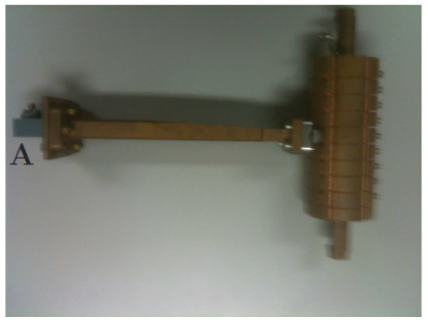
\includegraphics[width=0.48\textwidth]{3_1}}\quad
  \subfloat[Setup]{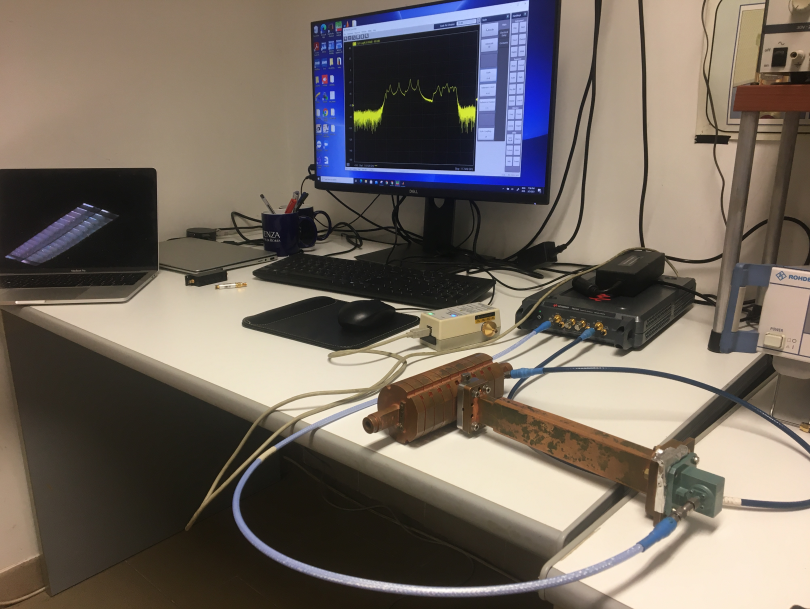
\includegraphics[width=0.48\textwidth]{3_1_2}}\\
\end{figure}

\end{frame}

\begin{frame}[t,fragile]{RF - Cavities (2) - Transmission Measurement}
\begin{itemize}
\item Identify different modes 
\item Calculated $Q$ from the \SI{3}{\dB} bandwidth: \num{3093}
\begin{itemize}
\item Center frequency: \SI{11.423}{\GHz}
\item Bandwidth: \SI{3.693}{\MHz}
\end{itemize}
\begin{figure}
  \centering\setcounter{subfigure}{0}
  \subfloat[All modes ($S_{21}$)]{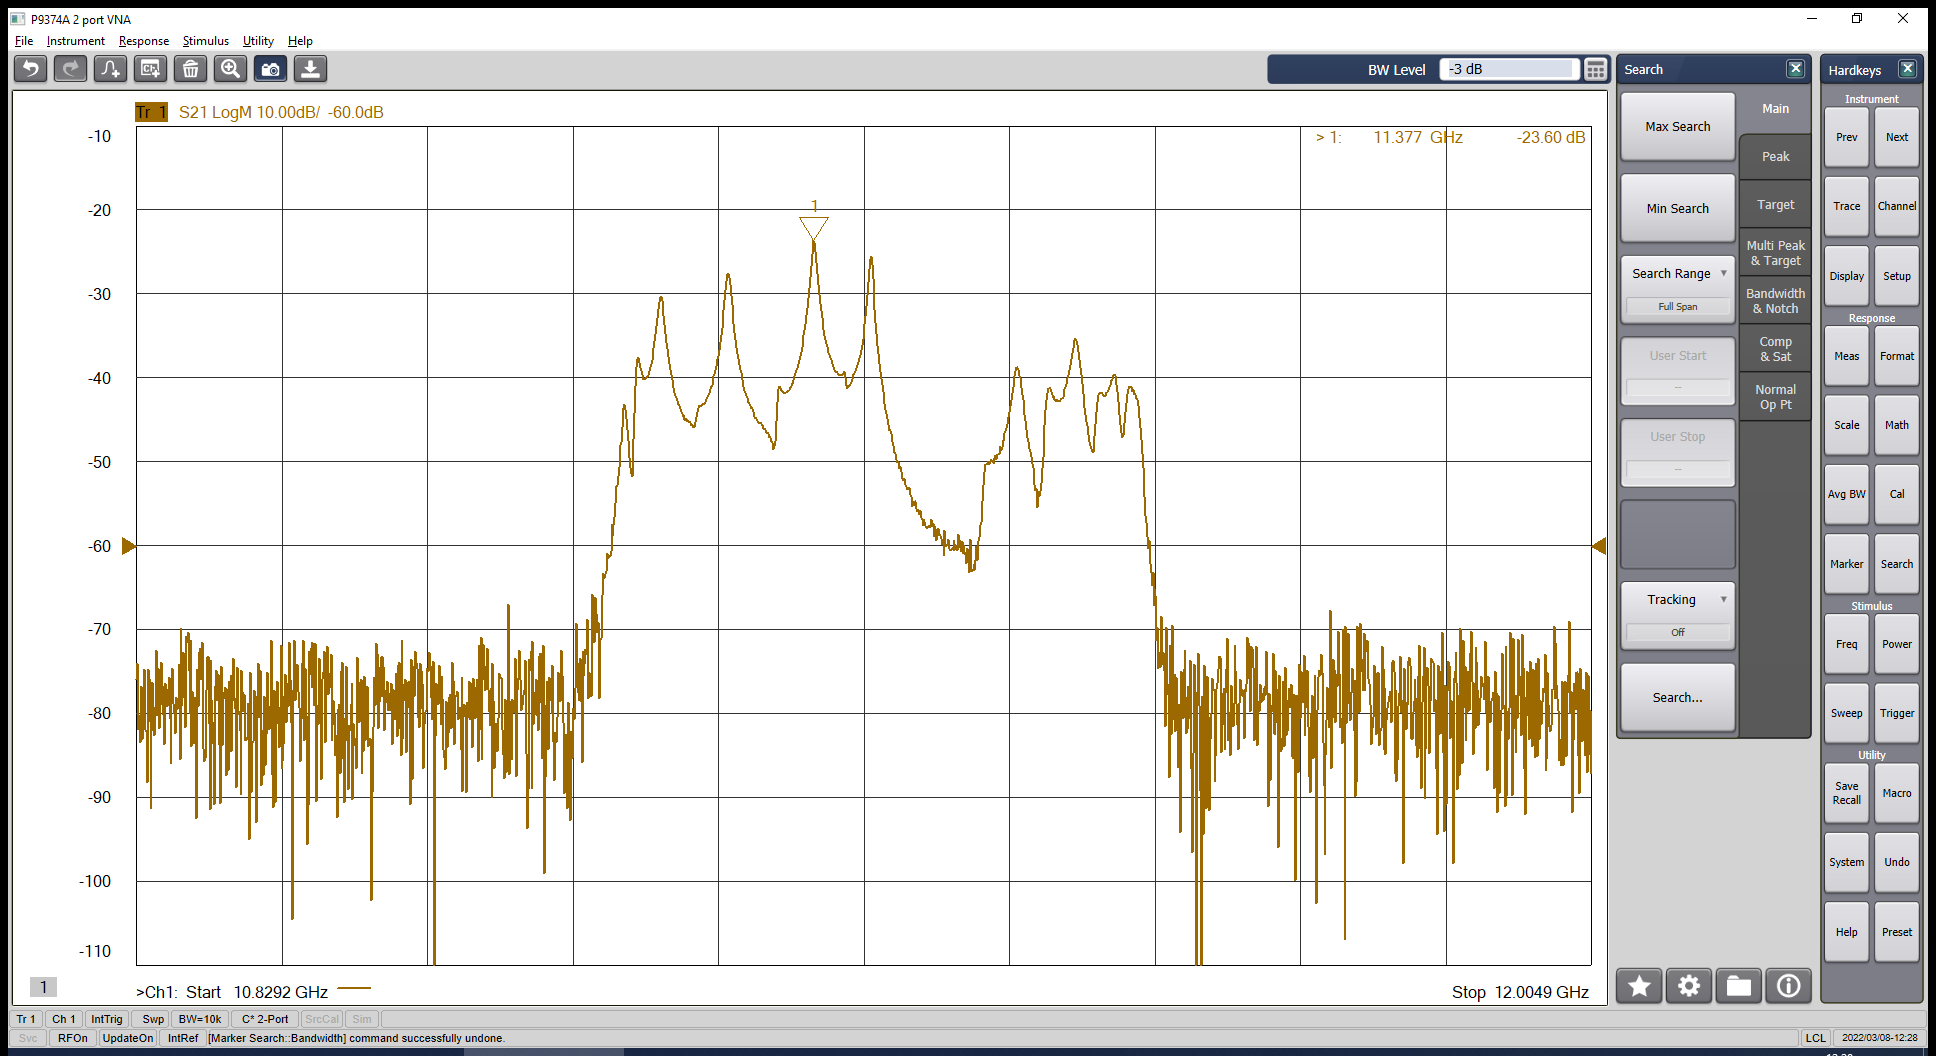
\includegraphics[width=0.45\textwidth]{3_S11_all_modes}}\quad
  \subfloat[$Q$ for a certain mode]{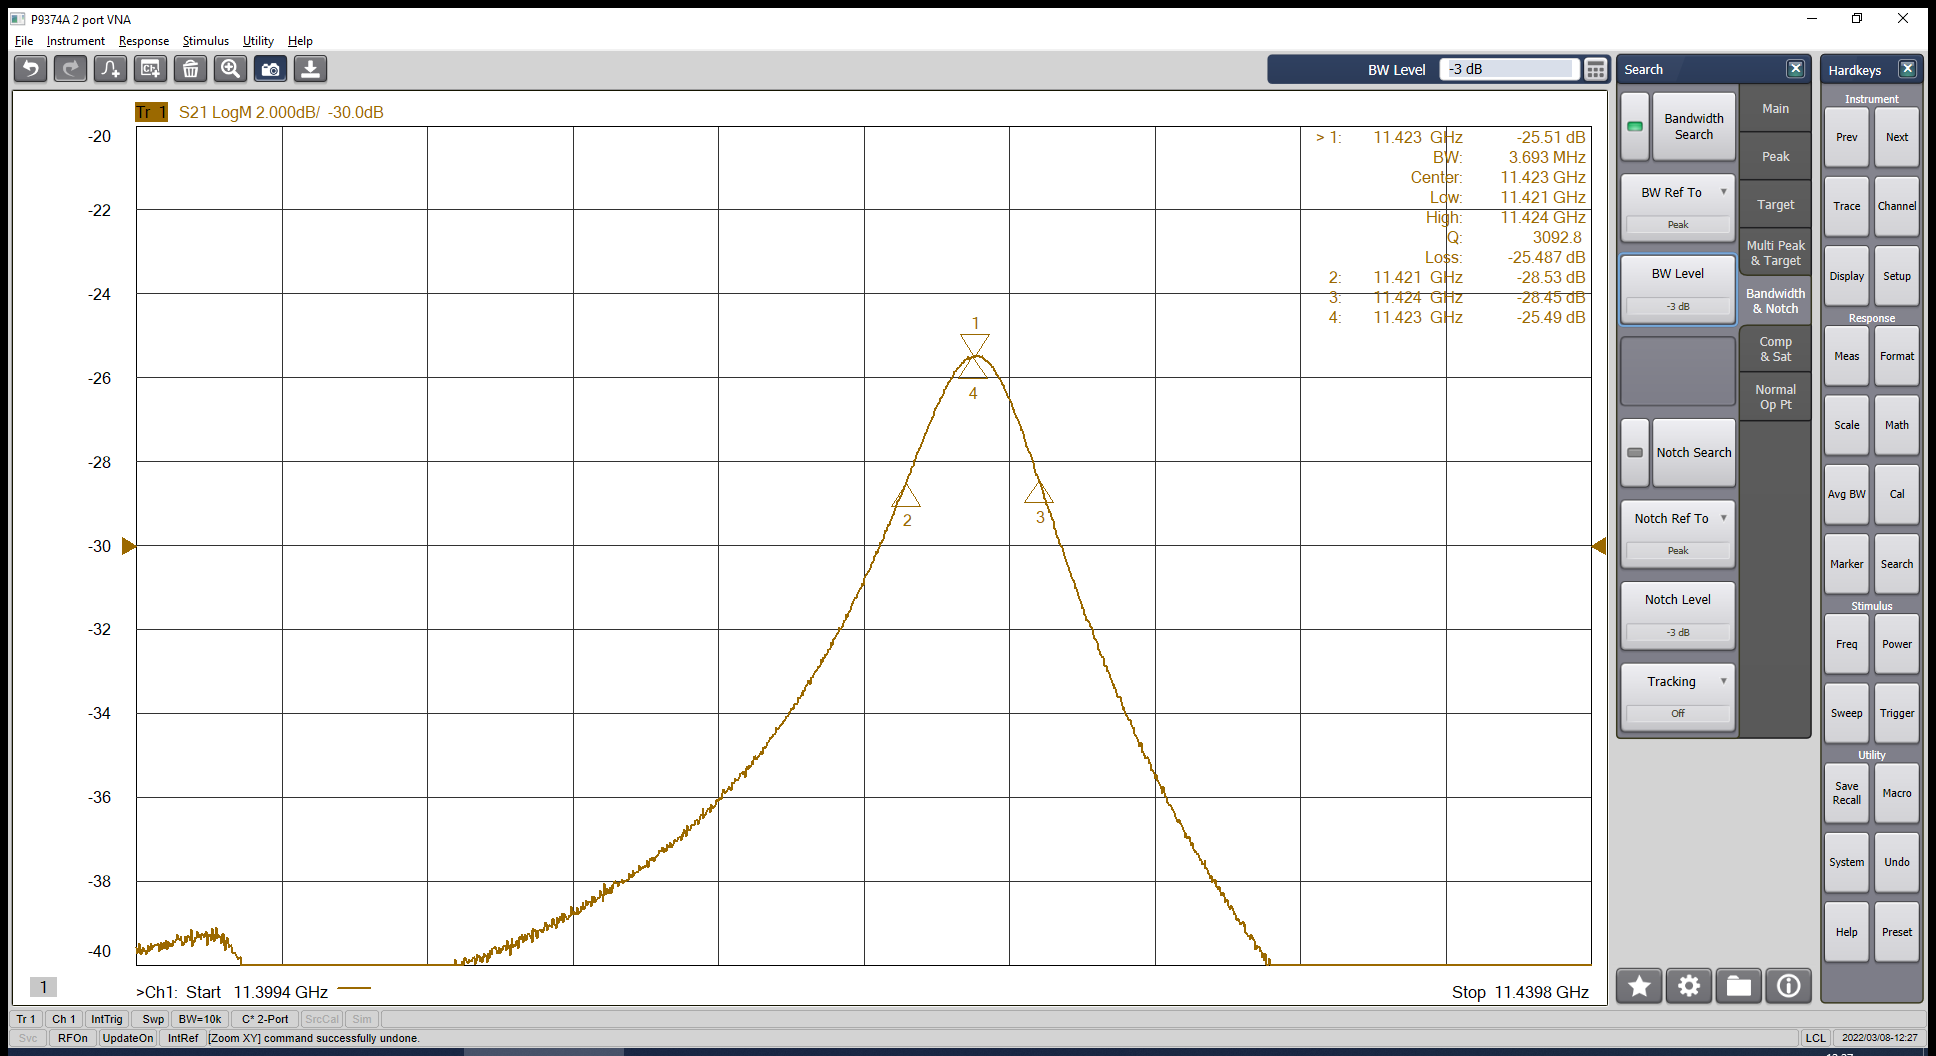
\includegraphics[width=0.45\textwidth]{3_S11_mode}}\\
\end{figure}
\end{itemize}
\end{frame}

\begin{frame}[t,fragile]{RF - Cavities (3) - Transmission Measurement}
\begin{itemize}
\item Identify SWR
\begin{itemize}
\item High SWR for high reflection
\item Low SWR for high transmission
\end{itemize}

\item Coupling ($S_{11}$ in Smith Chart)
\begin{itemize}
\item Under coupled
\end{itemize}
\end{itemize}
\begin{figure}
  \centering\setcounter{subfigure}{0}
  \subfloat[Under coupled: S21, S11, SWR]{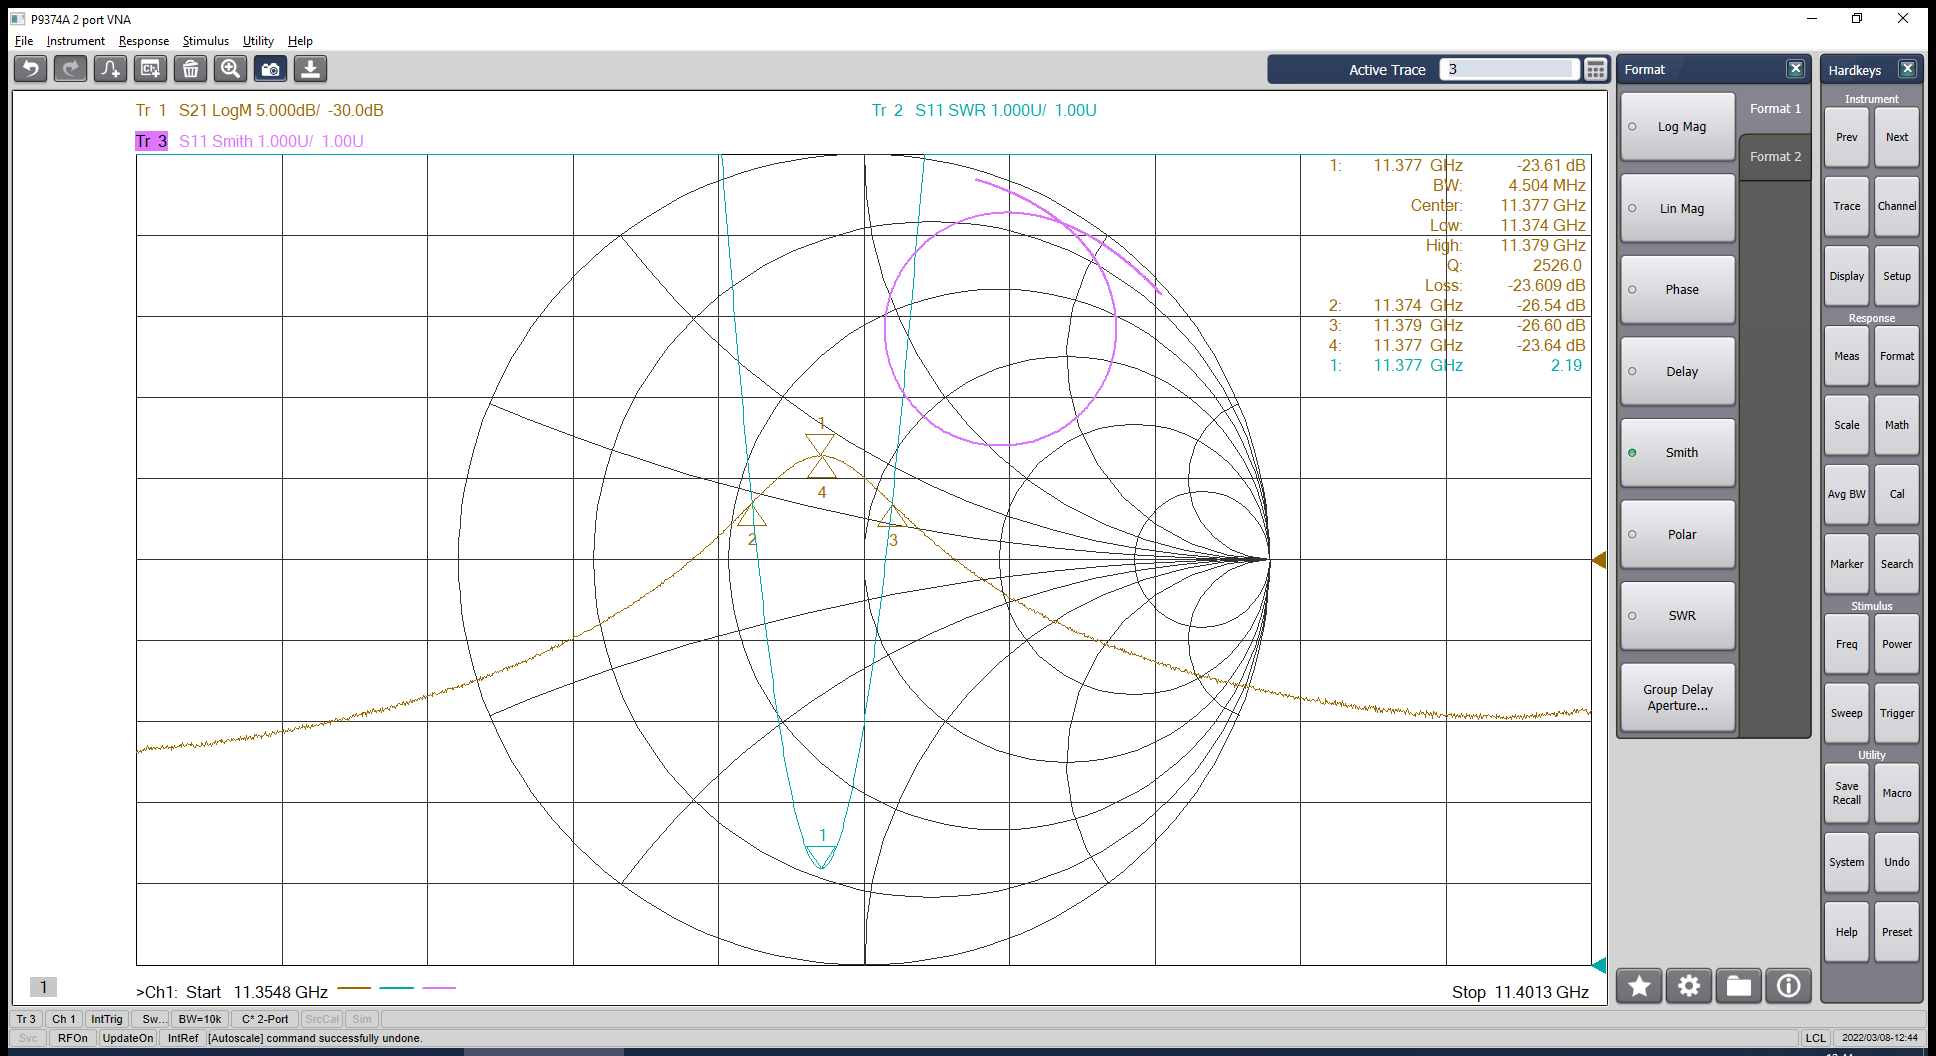
\includegraphics[width=0.48\textwidth]{3_comby_plot}}\quad
  \subfloat[Complete: S21, S11]{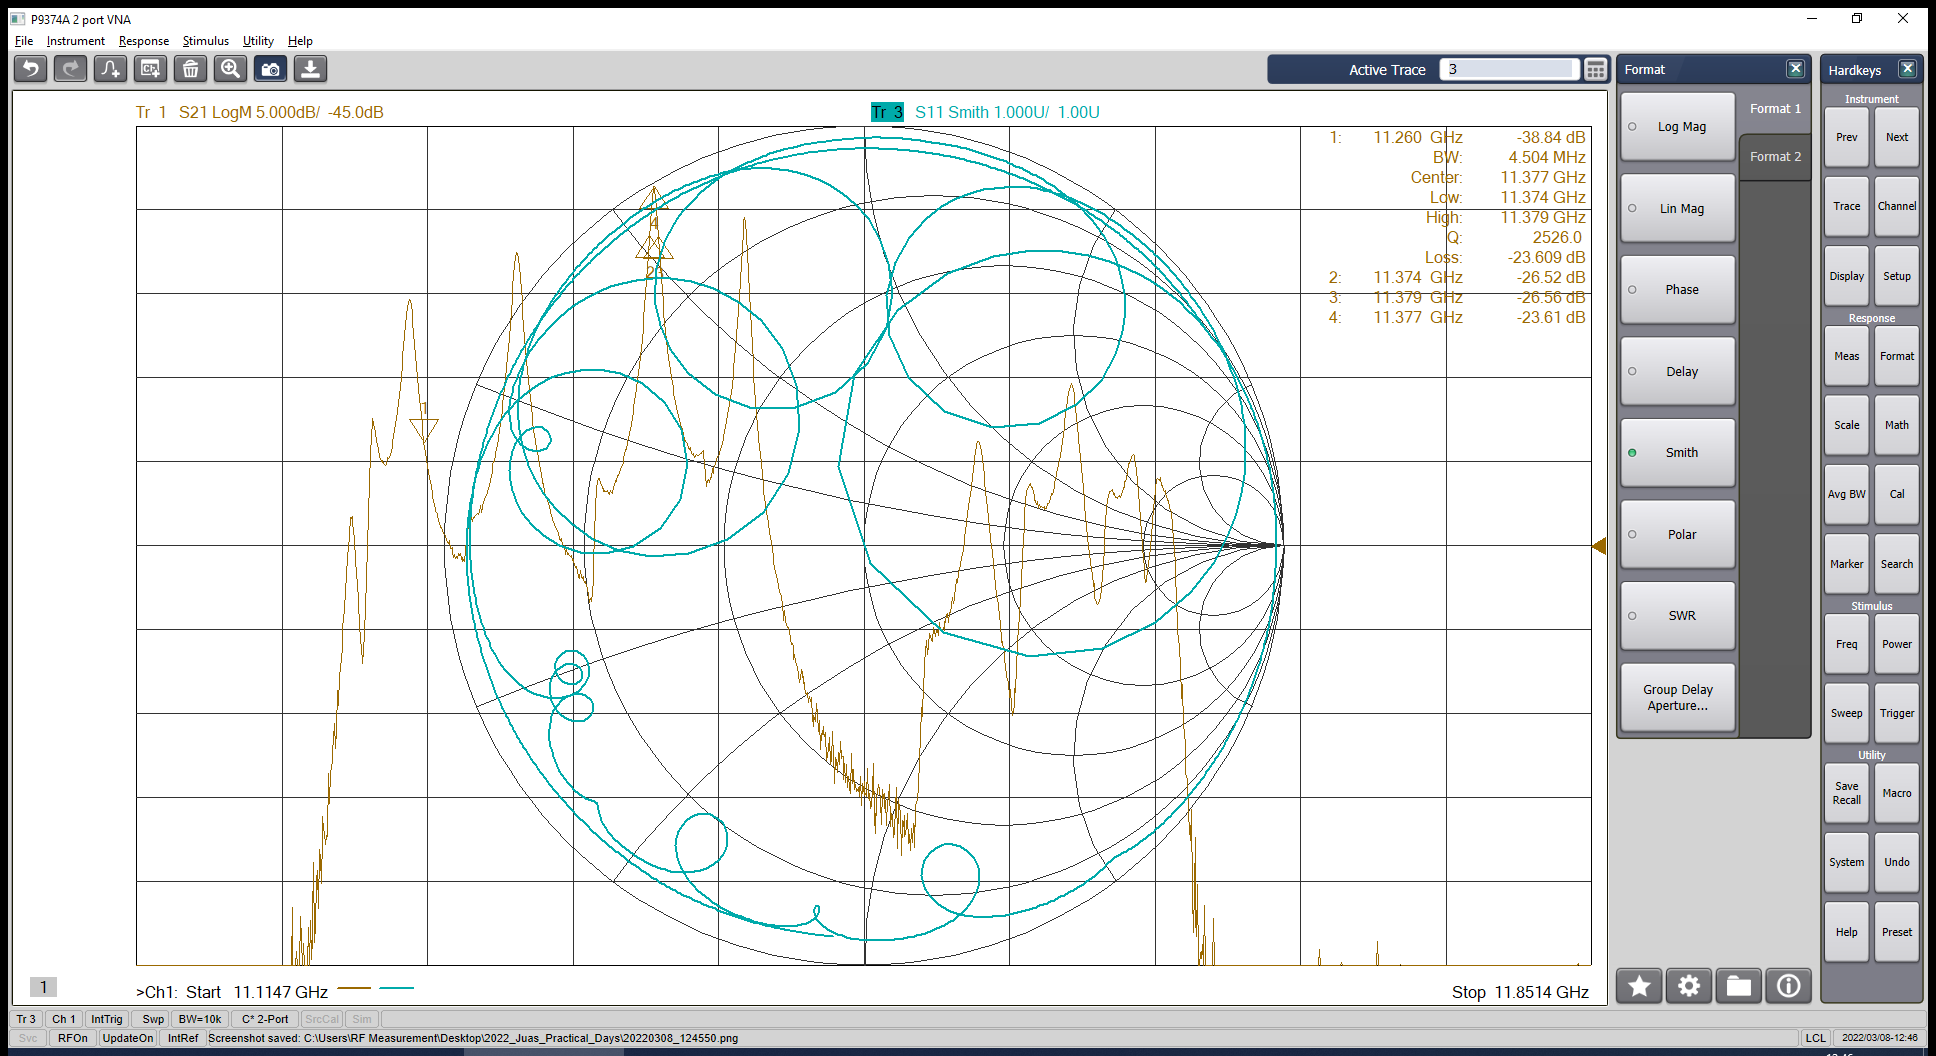
\includegraphics[width=0.48\textwidth]{3_comby_plot_all}}\\
\end{figure}

\end{frame}

\section{Afternoon Session}
\subsection{Instrument Review}
\begin{frame}[t,fragile]{Instruments and Calibration (Manfred Wendt)}
\begin{figure}
  \centering\setcounter{subfigure}{0}
  \subfloat[VNA]{\includegraphics[height=0.3\textwidth]{img/vna}}\;
  \subfloat[Electric Calibrator]{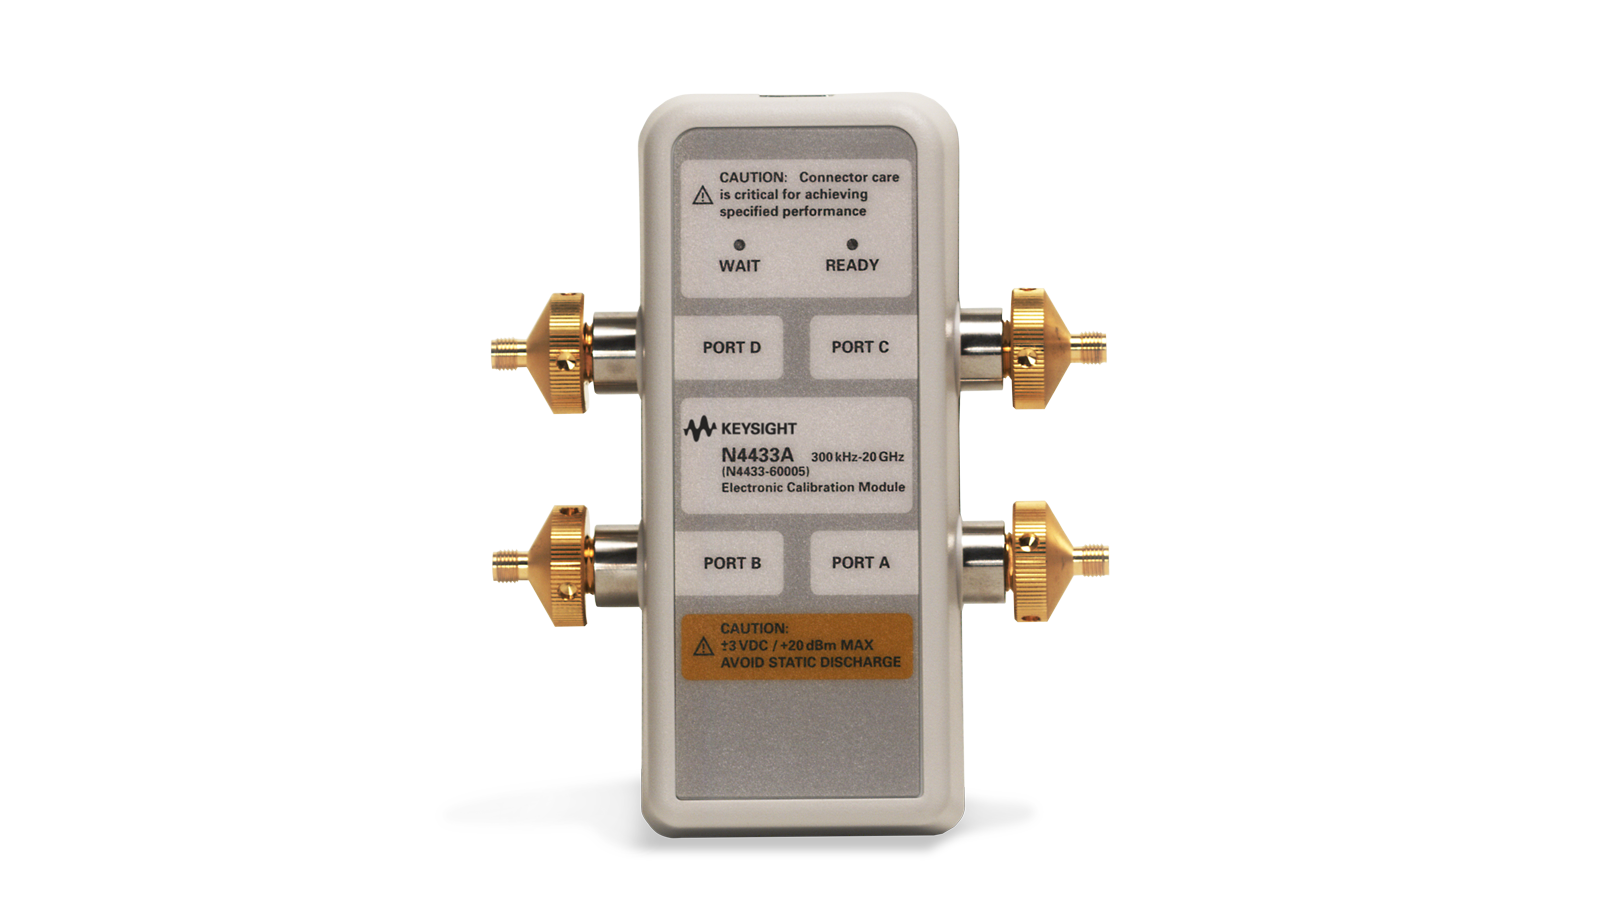
\includegraphics[height=0.3\textwidth]{img/cal}}
\end{figure}
\begin{itemize}
\item Vector Network Analyzer
\begin{itemize}
\item Constructs spectrum by narrowband downmixing
\item Can also display time domain via FFT
\end{itemize}
\item Calibrate before use!
\end{itemize}
\end{frame}

\subsection{Coupling of an RF Cavity}
\begin{frame}[t,fragile]{RF Cavity, Coupling, Smith Chart (Fritz Caspers)}
\begin{itemize}
\item  Two antennas in cavity
\begin{itemize}
\item Longitudinal field antenna
\item Coupling loop
\end{itemize}
\item Under-, over- and critical coupling

\begin{figure}
  \centering\setcounter{subfigure}{0}
  \subfloat[Under Coupled]{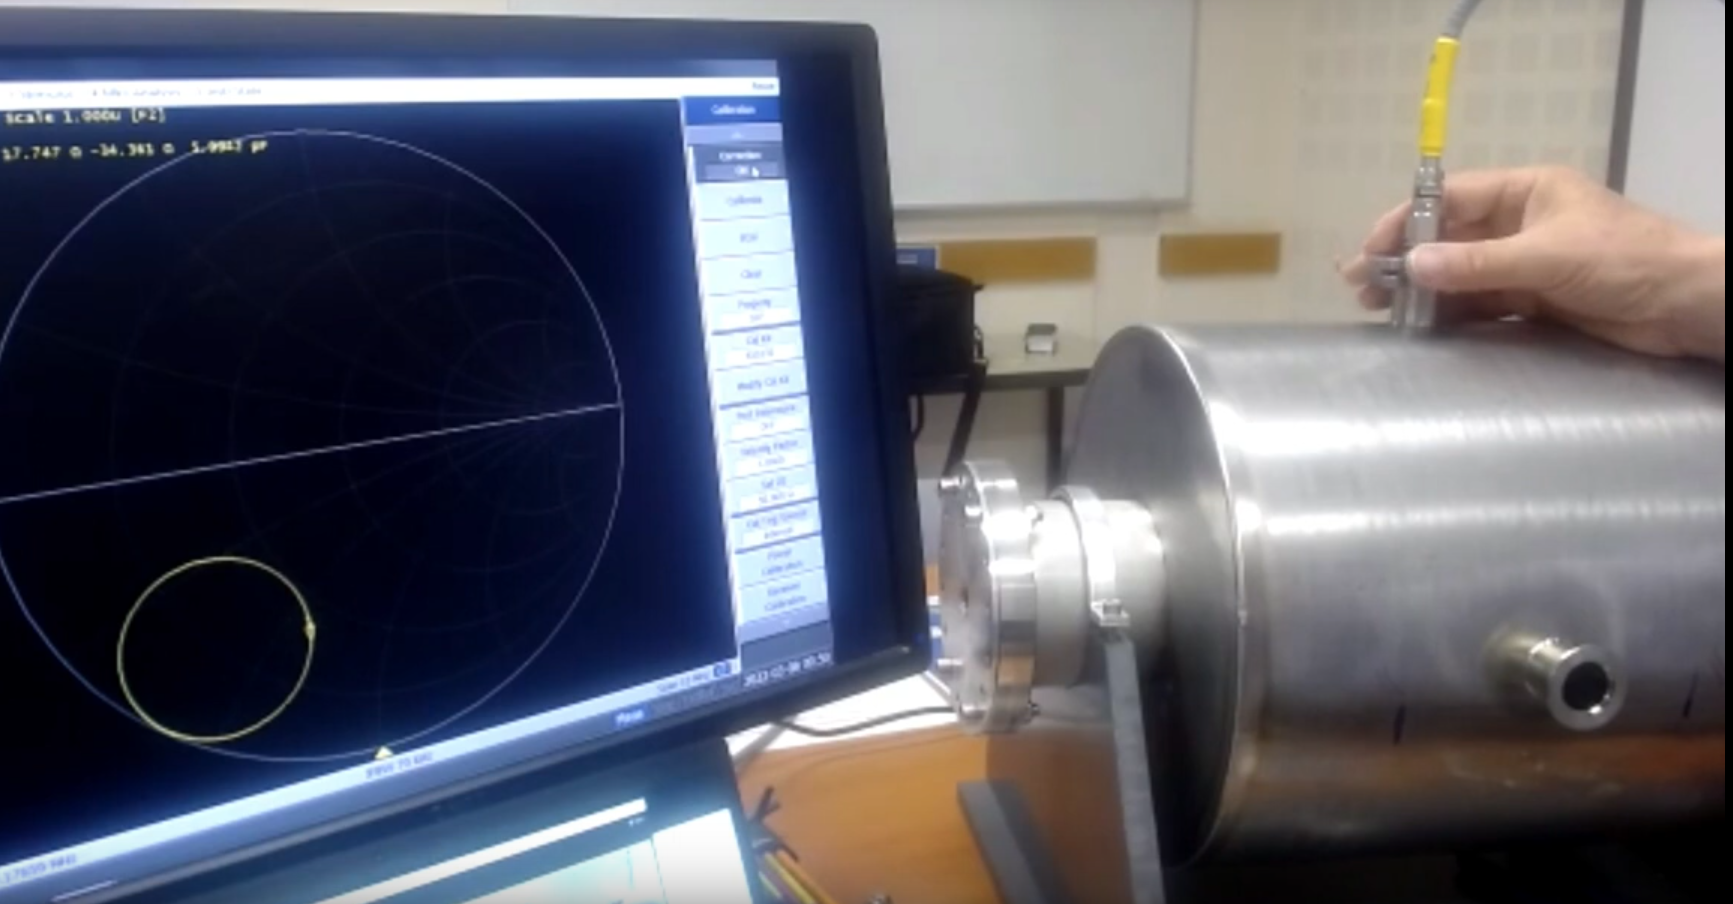
\includegraphics[height=0.16\textwidth]{img/cav_under.png}}\;
  \subfloat[Critically Coupled]{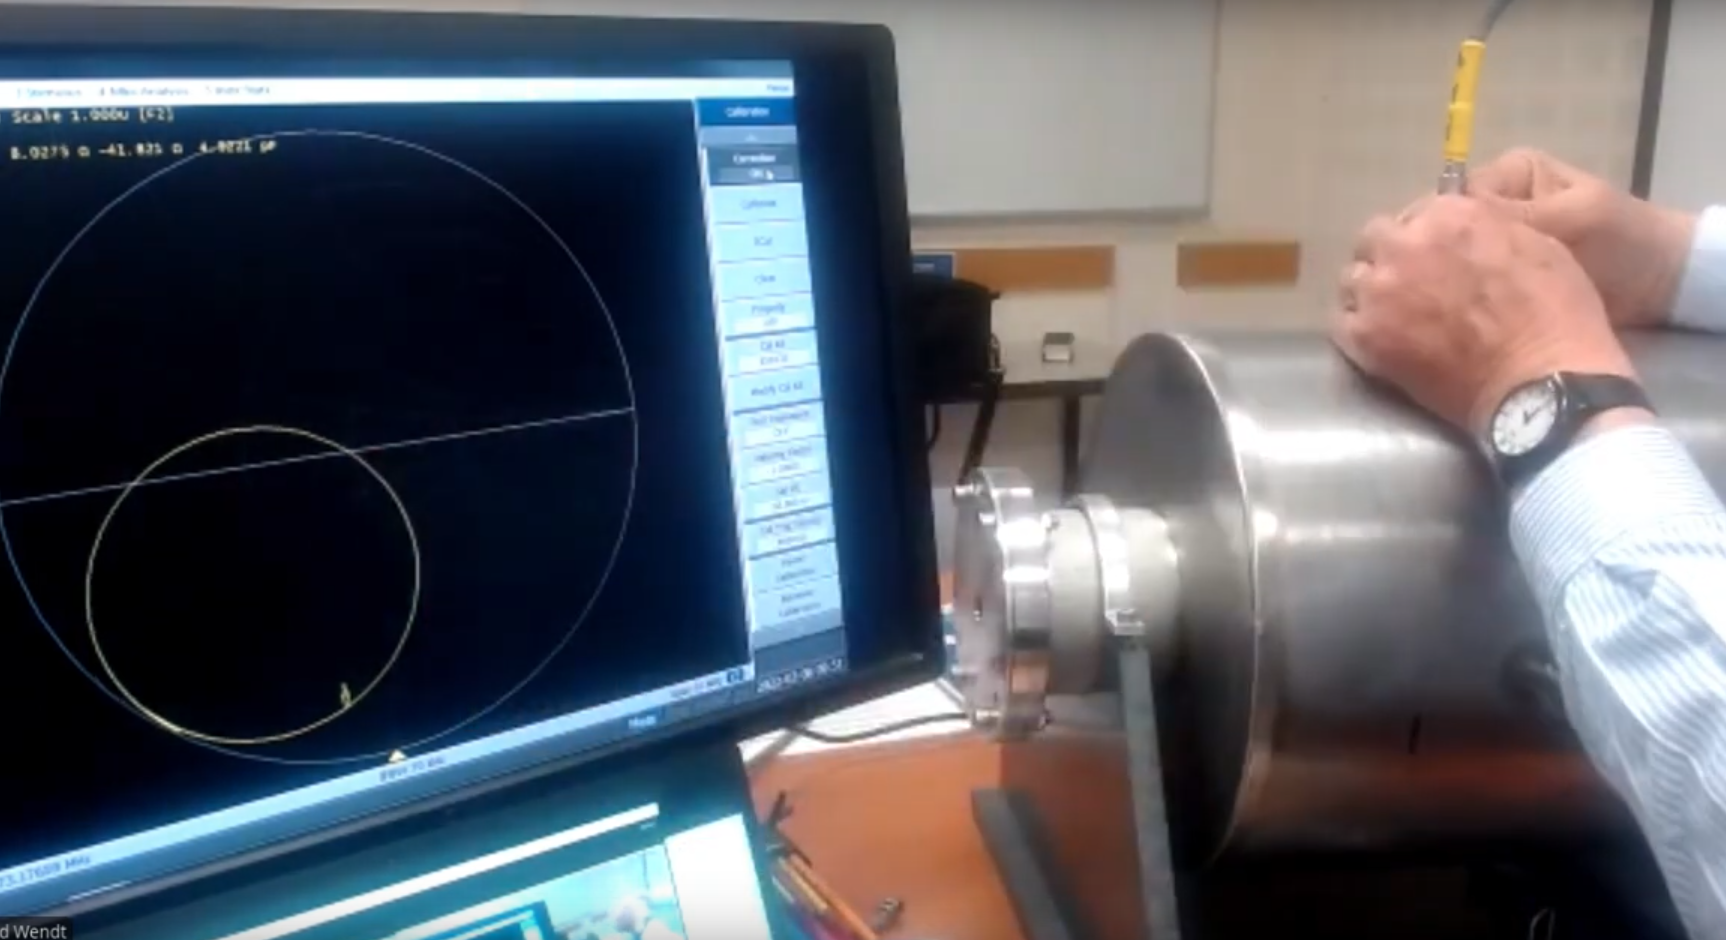
\includegraphics[height=0.16\textwidth]{img/cav_crit.png}}\;
  \subfloat[Over Coupled]{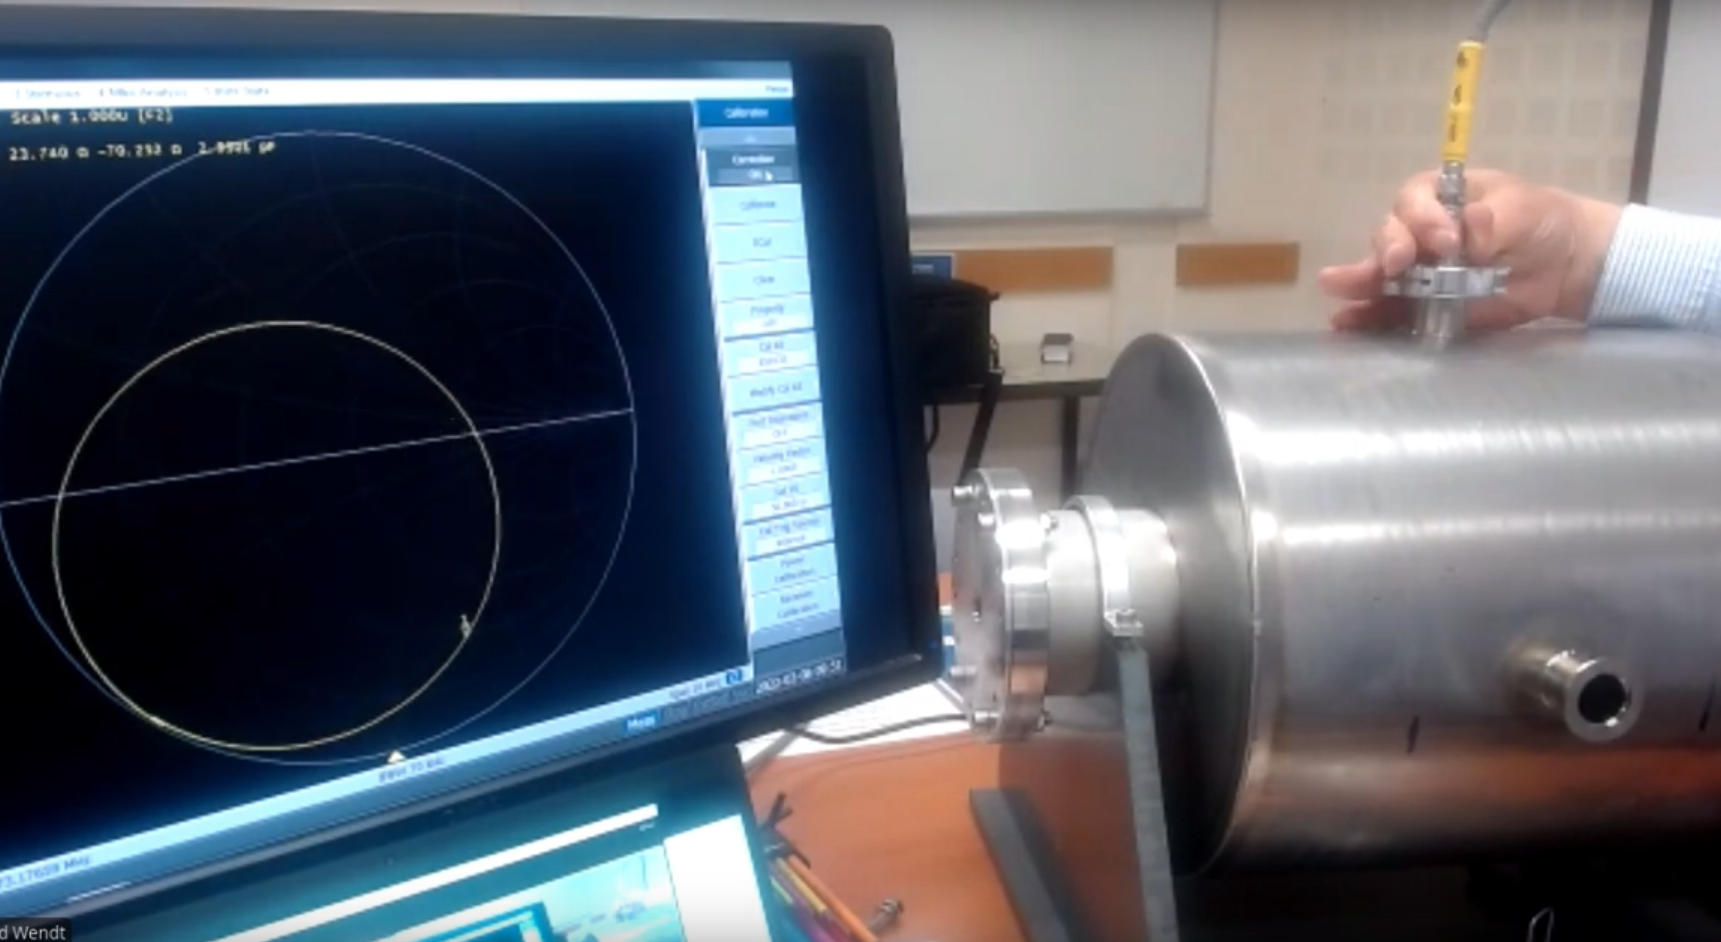
\includegraphics[height=0.16\textwidth]{img/cav_over.png}}
\end{figure}
\item Critical coupling desired ($\Gamma=0$)
\end{itemize}
\end{frame}

\section{Resume}
\begin{frame}[t,fragile]{Resume}
\begin{itemize}
\item Network Analyser
\begin{itemize}
\item Time and Frequency Domain
\item Scattering parameter, Impedance, SWR, phase
\item Calculation of $Q$, reflexion coefficient
\end{itemize}
\item Spectrum Analyser (Modulation)

\item Strip-line
\item Cavities (Coupling)
\end{itemize}
\begin{figure}
  \centering
  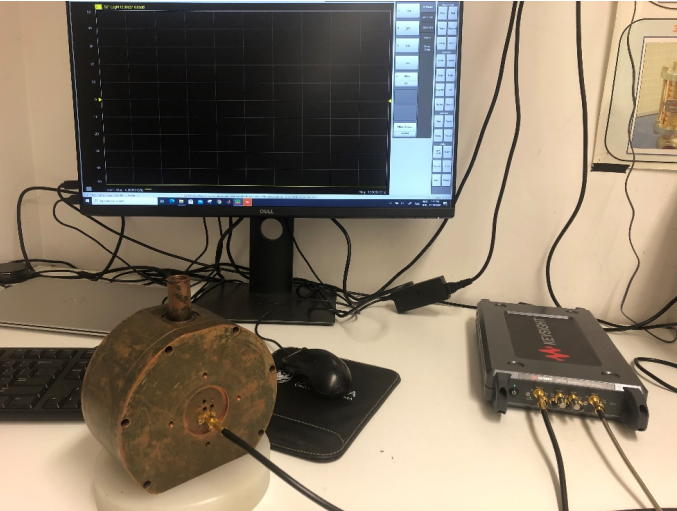
\includegraphics[width=0.32\textwidth]{4_resume}
  \caption{Cavity Setup}
\end{figure}
\end{frame}

\section{Appendix}
\begin{frame}[t,fragile]{Appendix (1) - Strip-line BPM}
\begin{figure}
  \centering\setcounter{subfigure}{0}
  \subfloat[S21: crosstalk]{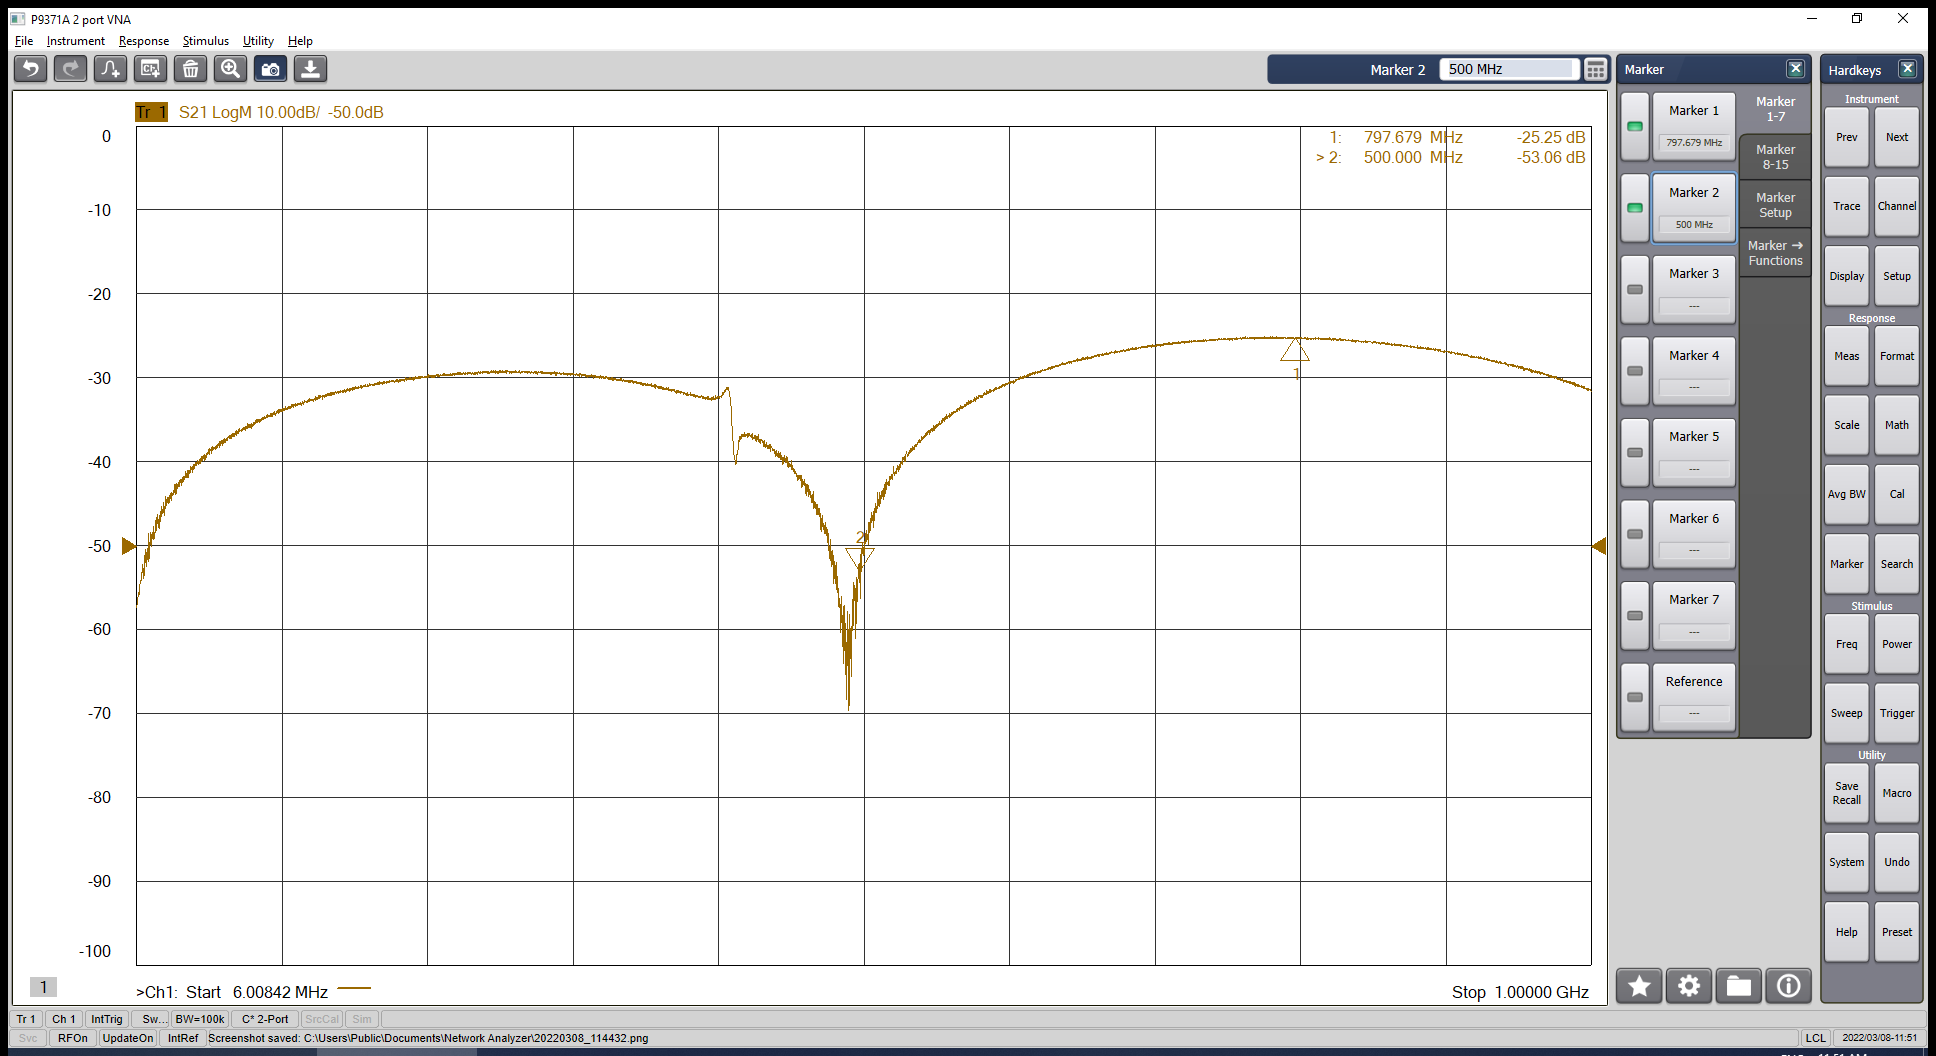
\includegraphics[width=0.45\textwidth]{2_crosstalk}}\quad
  \subfloat[Group delay]{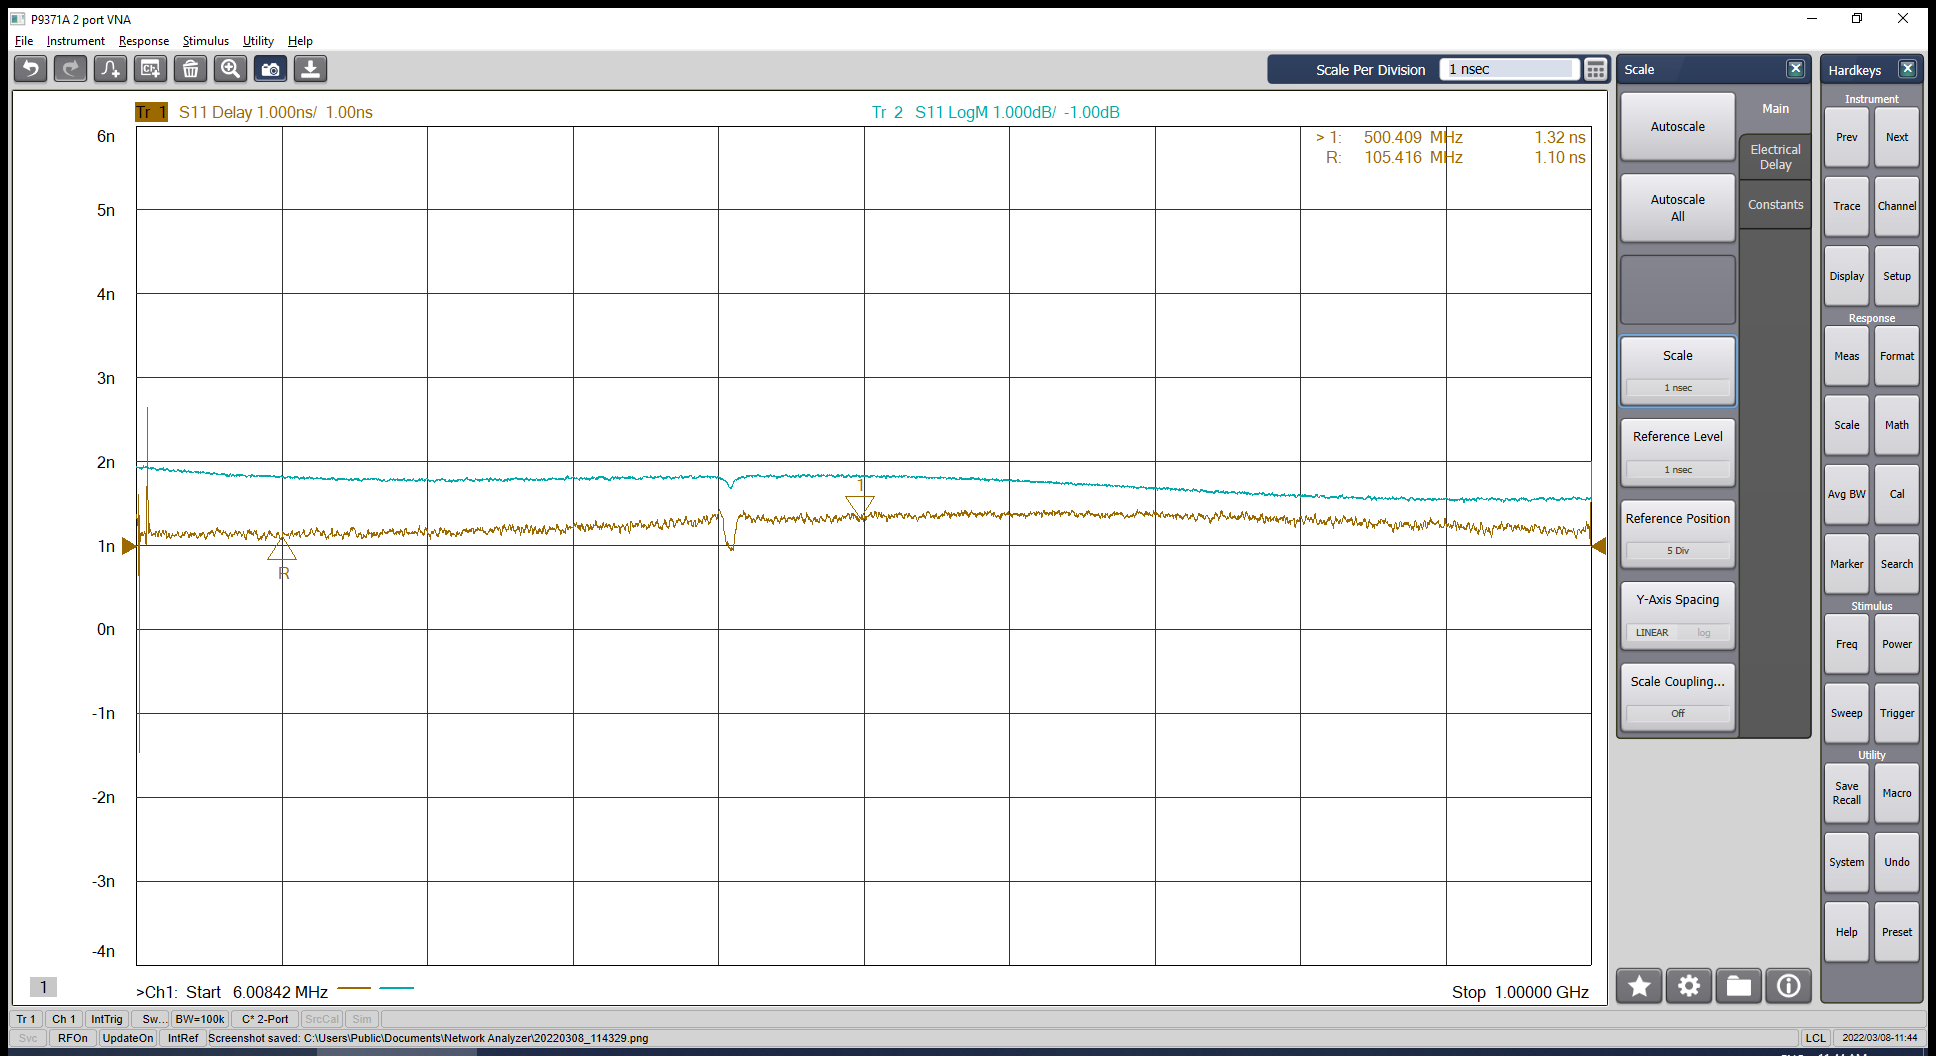
\includegraphics[width=0.45\textwidth]{2_group_delay}}\\
\end{figure}
\end{frame}

\begin{frame}[t,fragile]{Appendix (2) - Multi mode cavity}
\begin{figure}
  \centering\setcounter{subfigure}{0}
  \subfloat[S11, S21: for all modes]{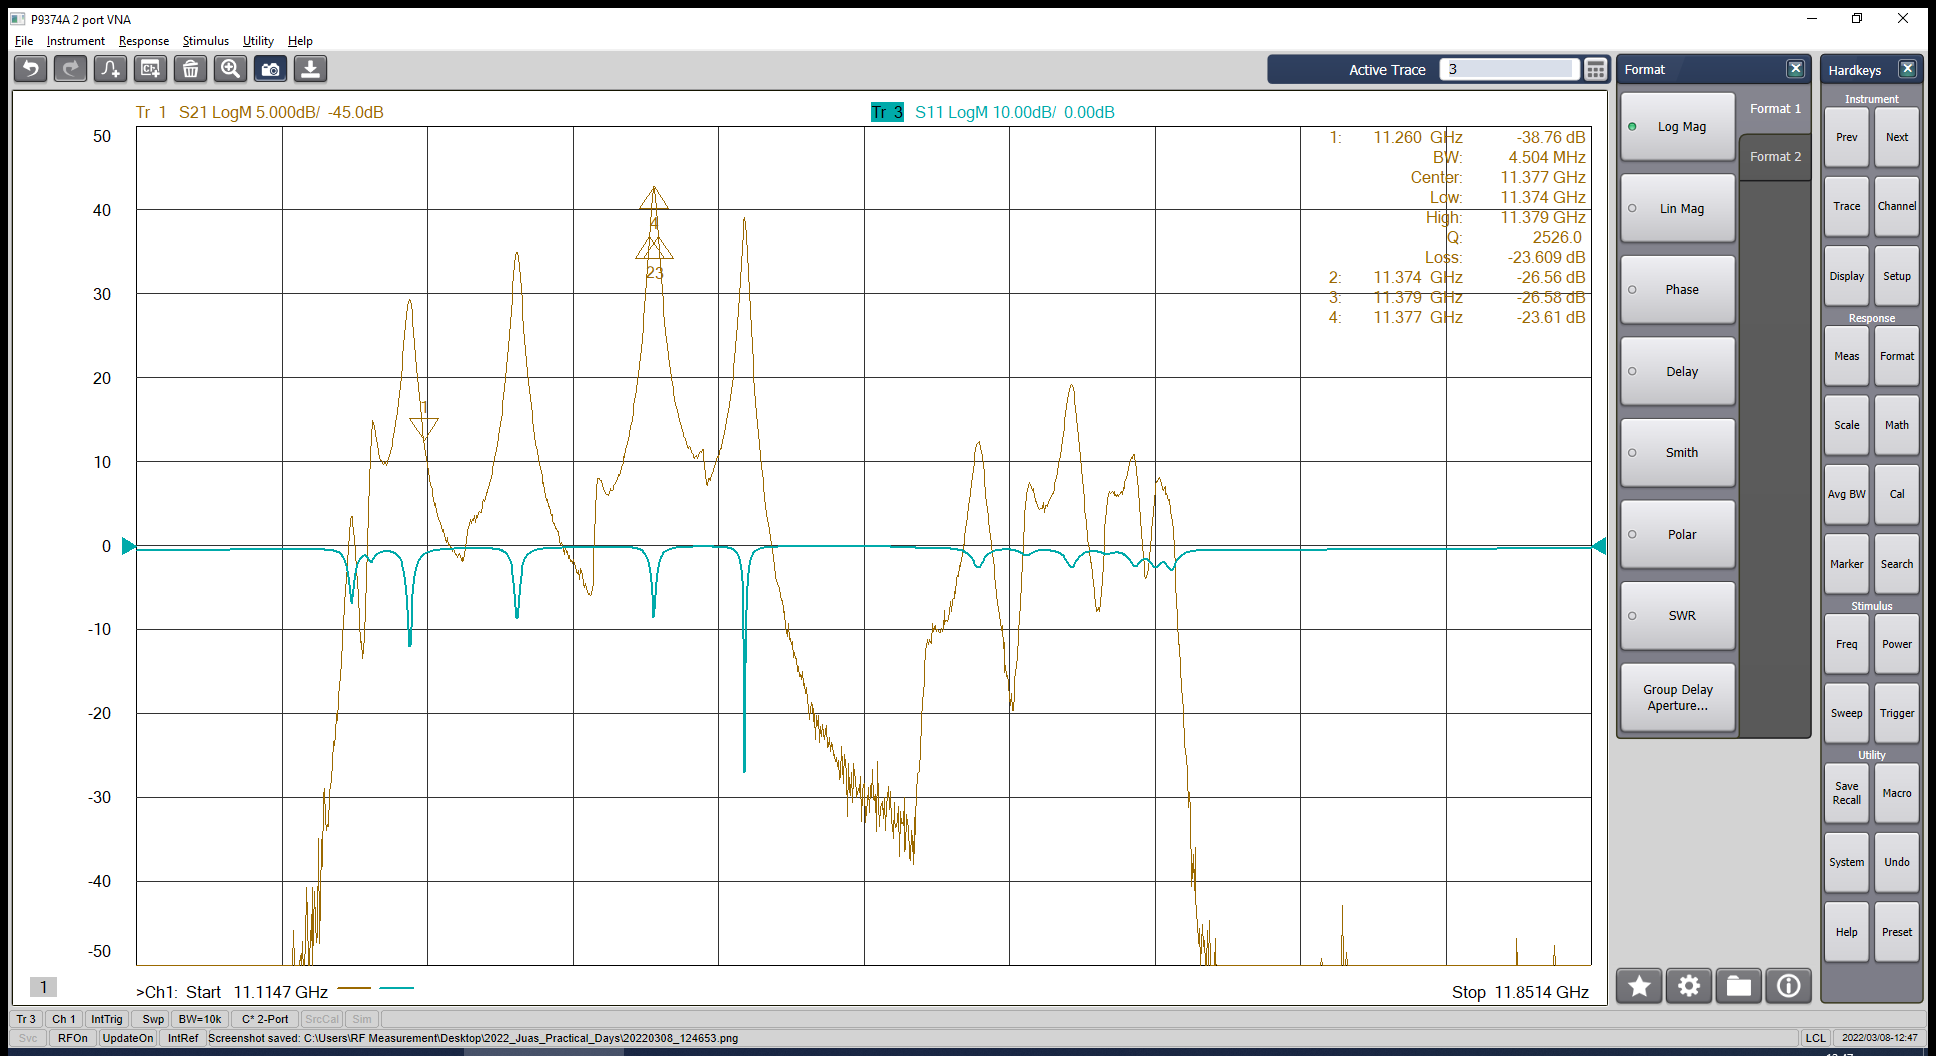
\includegraphics[width=0.45\textwidth]{5_3}}\quad
  \subfloat[S11, S21, S22]{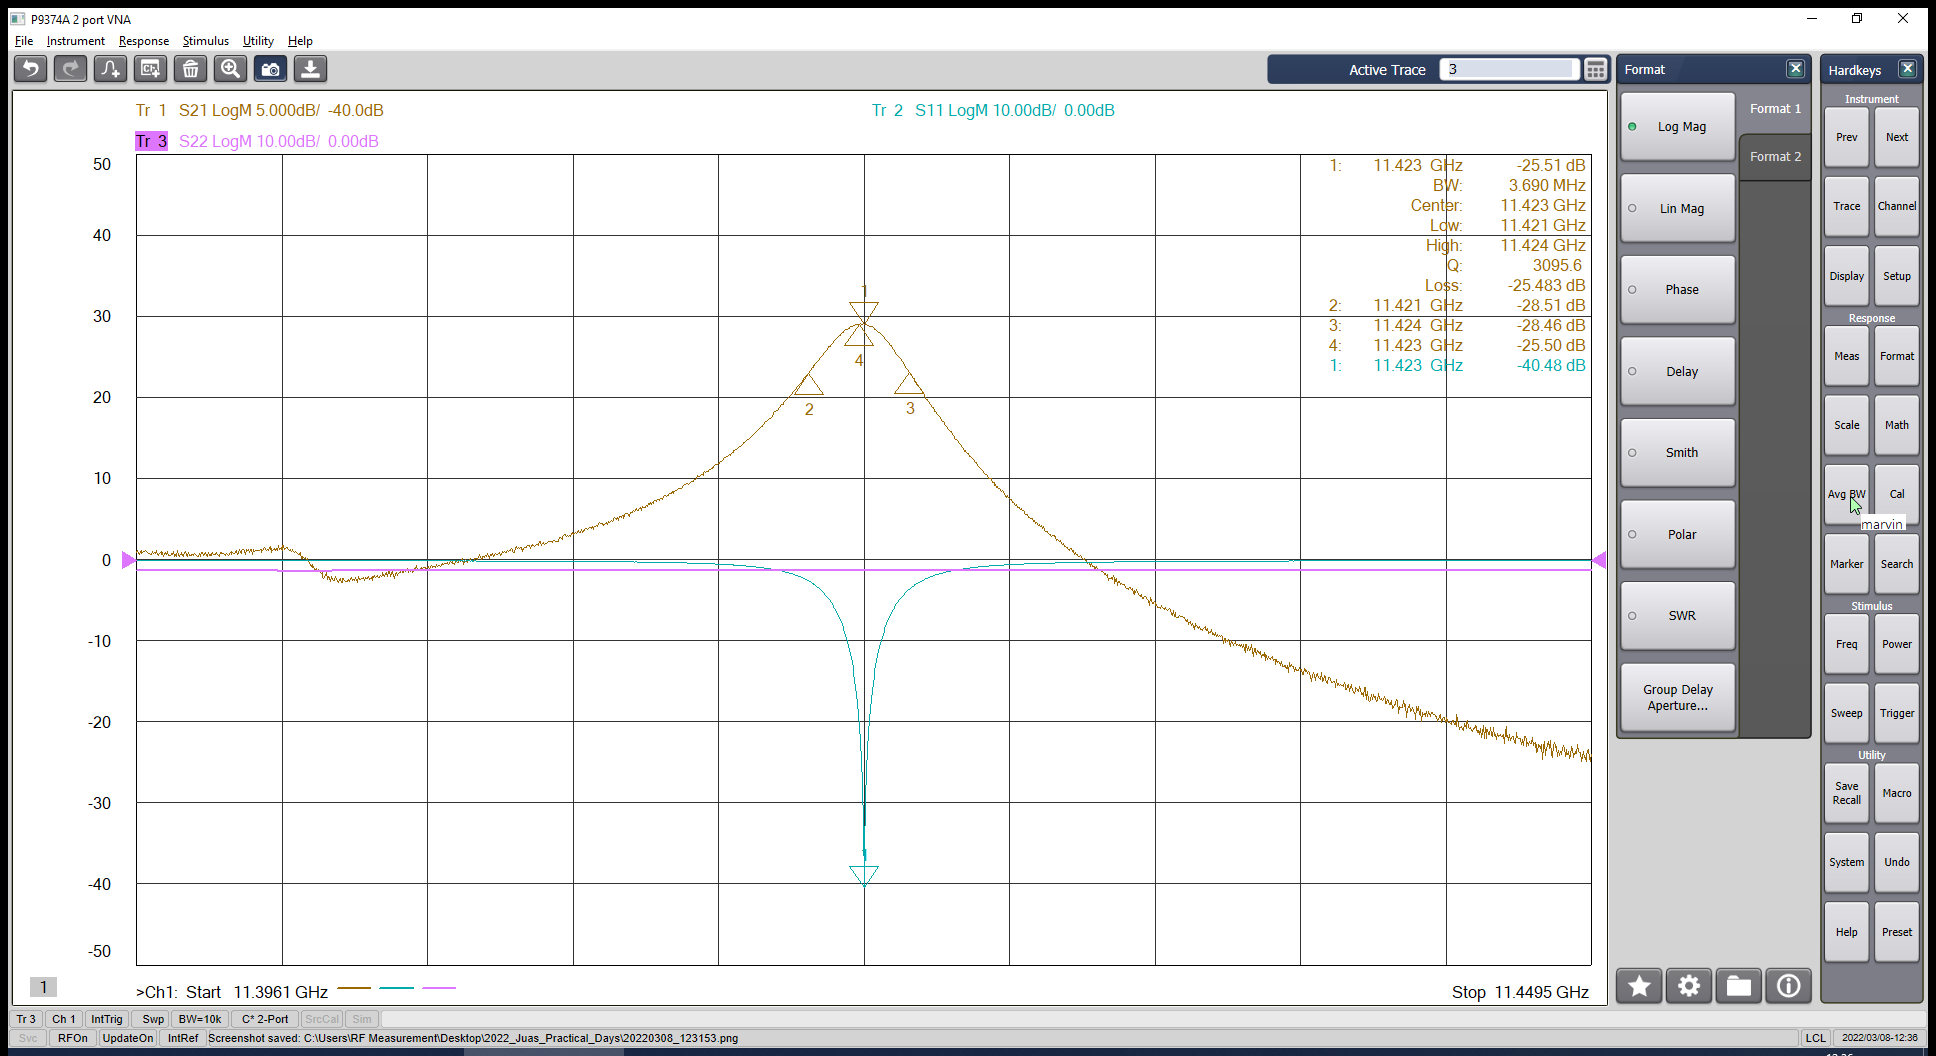
\includegraphics[width=0.45\textwidth]{5_3_2}}\\
\end{figure}
\end{frame}

\end{document}
